\documentclass{article}
\usepackage[T1]{fontenc}
\usepackage{lmodern}
\usepackage{graphicx}
\usepackage{amsmath,amssymb}
\usepackage[a4paper,margin=2cm]{geometry}
\usepackage[absolute,overlay]{textpos}
\setlength{\TPHorizModule}{1mm}
\setlength{\TPVertModule}{1mm}
\usepackage[indonesian]{babel}
\usepackage{hyperref}
\setlength{\emergencystretch}{2em}
\title{06-Serangan-pada-kriptografi-(2026)}
\author{pdf\_ppt\_to\_latex}
\date{}

\begin{document}

% --- unit llm 1 ---
% === Halaman 1 (llm) ===

\begin{center}
Bahan kuliah IF4020 Kriptografi

\Huge \textcolor{red}{07 - Serangan Terhadap Kriptografi}

\vspace{40mm}

\Large Oleh: Rinaldi M

\vspace{10mm}

\large Program Studi Teknik Informatika \\
Sekolah Teknik Elektro dan Informatika \\
Institut Teknologi Bandung \\
2026
\end{center}

\newpage

% --- unit llm 2 ---
% === Halaman 2 (llm) ===

\section*{Pendahuluan}

\begin{itemize}
    \item Keseluruhan \textit{point} dari kriptografi adalah menjaga kerahasiaan pesan atau kunci dari pihak ketiga. Pihak ketiga: musuh, lawan, penyadap, kriptanalisis (\textit{cryptanalyst}).
    \item Pihak lawan berusaha memecahkan cipherteks dengan melakukan serangan terhadap sistem kriptografi.
    \item Tujuan serangan adalah untuk mengungkap plainteks dari cipherteks atau mendapatkan kunci dekripsi, sehingga kunci dekripsi dapat digunakan untuk mendekripsi potongan cipherteks lainnya.
\end{itemize}

\newpage

% --- unit llm 3 ---
% === Halaman 3 (llm) ===

\section*{Serangan (\textit{attack})}

\begin{itemize}
    \item \textbf{Serangan} diartikan sebagai setiap usaha (\textit{attempt}) atau percobaan yang dilakukan oleh pihak lawan untuk menemukan kunci atau menemukan plainteks dari cipherteksnya.
    \item Asumsi: penyerang mengetahui algoritma kriptografi yang digunakan
\end{itemize}

\textbf{Prinsip Kerckhoff}: Semua algoritma kriptografi harus publik; hanya kunci yang rahasia.

Jadi, keamanan sistem kriptografi terletak pada \textcolor{red}{kunci}!

\newpage

% --- unit llm 4 ---
% === Halaman 4 (llm) ===

\section*{Jenis-jenis Serangan (1)}

\vspace{133.06mm}

\begin{itemize}
    \item Berdasarkan ketersediaan informasi yang digunakan untuk menyerang sistem kriptografi:
\end{itemize}

\begin{enumerate}
    \item Chipertext-only attack
    \item Known-plaintext attack
    \item Chosen-plaintext attack
    \item Adaptive-chosen-plaintext attack
    \item Chosen-chipertext attack
\end{enumerate}

\vspace{10mm}

% deskripsi: Komik dua panel yang membandingkan imajinasi seorang 'crypto nerd' tentang menyerang sistem enkripsi RSA dengan komputer mahal versus realitas serangan fisik (pemerasan) untuk mendapatkan kata sandi.
% bbox normalisasi: [0.4770, 0.3560, 0.9330, 0.8040]
\begin{textblock*}{95.76mm}(100.17mm,105.73mm)
\noindent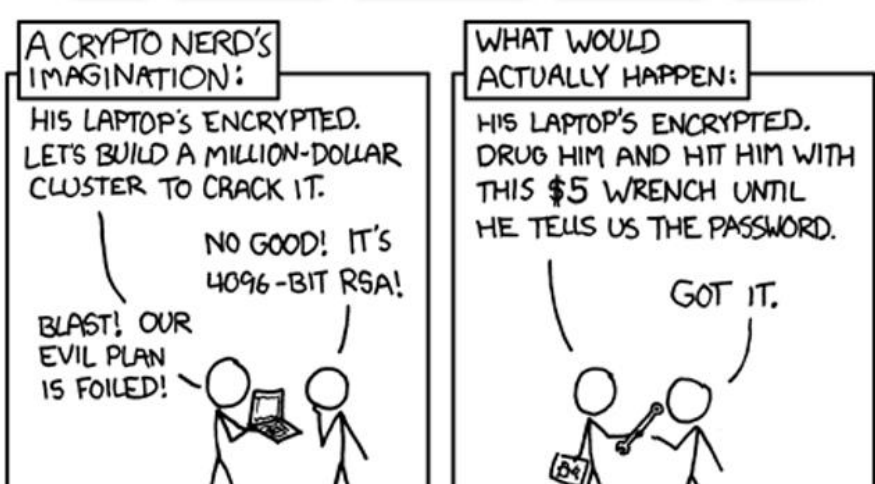
\includegraphics[width=95.76mm,height=133.06mm]{images/llm/page_004_img_01.png}%
\end{textblock*}

\newpage

% --- unit llm 5 ---
% === Halaman 5 (llm) ===

\section*{1. Chipertext-only attack}

Kriptanalis hanya memiliki cipherteks saja. Ini serangan paling sulit karena informasi yang diperoleh hanya sedikit (cipherteks saja).

Teknik yang digunakan: \textit{exhaustive key search}, terkaan, \textit{metode} analisis frekuensi, dsb.

Diberikan: \[ C_1 = E_k(P_1), \quad C_2 = E_k(P_2), \quad ..., \quad C_i = E_k(P_i) \]

\vspace{71.28mm}

Deduksi: \[ P_1, P_2, \dots, P_i \text{ atau } k \text{ untuk mendapatkan} \]
\[ P_{i+1} \text{ dari } C_{i+1} = E_k(P_{i+1}). \]

\vspace{10mm}

% deskripsi: Diagram ilustrasi serangan Ciphertext-Only Attack yang menunjukkan Alice mengirim ciphertext ke Bob, dan Eve mencegat ciphertext tersebut untuk dianalisis guna mendapatkan plaintext.
% bbox normalisasi: [0.5200, 0.6300, 0.9800, 0.8700]
\begin{textblock*}{96.60mm}(109.20mm,187.11mm)
\noindent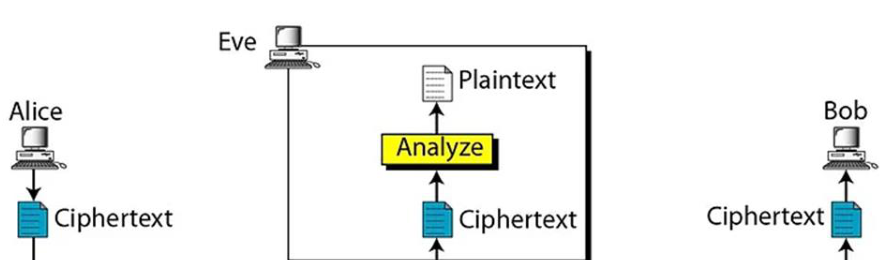
\includegraphics[width=96.60mm,height=71.28mm]{images/llm/page_005_img_01.png}%
\end{textblock*}

\newpage

% --- unit llm 6 ---
% === Halaman 6 (llm) ===

hQIMAw3Jn/nLK/38ARAAsSXLDhCtzUYKMptNxZImJXwhhIRm3QxfuyHjJ93ASyLE\ne+6ABkuyFLJhiKryxp/Jms/a LMPFf7hx2aTgovagaPzTwTV1jo6If2mhdC16eed\n1iz7C0f6jHIqq9d8g0bWDyvEleip5LNDTX3Xp2Csx50jBR2wckrUt111Xyj8G0H\n4DQUYBinRMJvJULJJC/acGvgOze66pHuRGScXXhDScefjXenh/XejSYTo7aMi+Es7\nDCCd49zh6ZLDQN6BLN9q2oFI8QiHq2y1Qjbat1dWi/4yYW1KzCLKRSm8eo/gNCdL\nh9MncBXBsFgbvbu67CDZ9GO5gezOn3LzQpo8jHrZ6/6/uMKuEZjW3RCo0T754f\nE5zYelwUgtws/1mQ2w5PQF/89bpshtDSYuL1fZgzrsE6DwophuCri5zwCGbEKlsI\nq6REIETFbz2aCL4N2pZVunCIEuOPz0gEB6+M9egdpyMxSomEQbVG3AH7SalAtEguP\nT/MCxI0bZCHuP EKT8ls bSRdN xTWMUXQt3XpL0bGCCRMLKSOWyFd iDnNrK fbWk\niiqw9hx4Q9Cjg7x7XRJnVgwoEReIFNmYSBfLVpS xEoU6F dByhdq SFekin4Wnkmdw\nqrS18fjIW/kzV27z u0beKky9ubBox76yjLro9KUQms3em03kc6459g5TDIz0qF\nAgwDrosDP2BeYQBD/9H5VKFw0an5j5MX1JpOSBAqNGKw2bcEFnwJfk0DD1lyHD\nowHig7gDowCS+5y/pf56v36HkpzJZATKqGOryKVxmQOxU913Yn5Pc fw8iFxlrfcG\nywzkJh/BRDQ/uy5fhGc/PbSm6iLv/SkkWTK8PSUD+glyZyK0W7WkM9QYS20E71Q\nqbwpNiy57reWkUWCOE4QmKqqpe7NXXM0eLT912D0hG21thyvTvVspkpxs zl8+HMJV\nM2LMcY2FmmZWAJSdxsQs9NQdyvcJX2D80a89W QyXmp7MPXL7BQfoQNPndmn60Bi\n0EQojoeMRNh14XNnHMJPjxW7m34R2hGtvnd3NG8iFrtoCOV JXqXUu3N+9T2sNe/bS8\n\n\begin{center}\large \textcolor{red}{Cipherteks}\end{center}

\newpage

% --- unit llm 7 ---
% === Halaman 7 (llm) ===

\begin{itemize}
    \item Contoh pada Caesar Cipher, penyerang hanya memiliki cipherteks berikut:
    
    KHOORZRUOG
    
    Penyerang tidak tahu kunci (pergeseran berapa huruf), hanya punya cipherteks itu saja.
\end{itemize}

Namun karena Caesar cipher hanya punya 25 kemungkinan pergeseran huruf, penyerang bisa mencoba semua pergeseran (\textit{brute force}).

Saat dicoba pergeseran 3 huruf ke kiri, diperoleh plainteks:

HELLOWORLD

Serangan berhasil menemukan kunci dan memecahkan cipherteks!

\newpage

% --- unit llm 8 ---
% === Halaman 8 (llm) ===

\section*{2. Known-plaintext attack}

Diberikan sejumlah pasangan plainteks dan cipherteks yang berkoresponden:

\[ P_1 \text{ dan } C_1 = E_k(P_1), \quad P_2 \text{ dan } C_2 = E_k(P_2), \quad \dots, \quad P_i \text{ dan } C_i = E_k(P_i) \]

Deduksi: $k$ untuk mendapatkan $P_{i+1}$ dari $C_{i+1} = E_k(P_{i+1})$.

\vspace{10mm}

Sumber: \url{https://www.hackers.arise.com/post/2019/04/30/cryptography-basics-part-2-attack-models-for-cryptanalysis}

% deskripsi: Diagram ilustrasi Known-Plaintext Attack yang menunjukkan Eve menganalisis pasangan Plaintext dan Ciphertext sebelumnya untuk memecahkan pesan yang dikirim dari Alice ke Bob.
% bbox normalisasi: [0.2180, 0.5970, 0.7210, 0.8430]
\begin{textblock*}{105.63mm}(45.78mm,177.31mm)
\noindent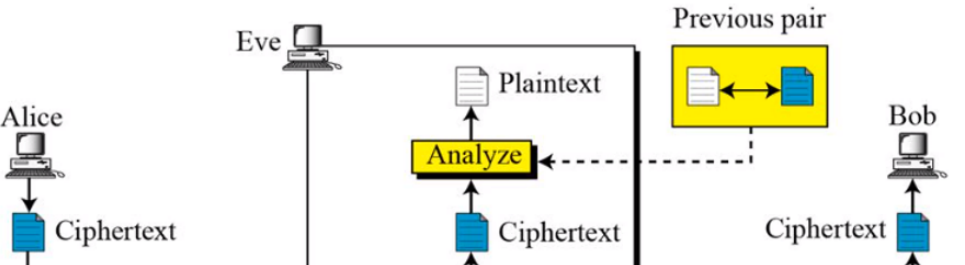
\includegraphics[width=105.63mm,height=73.06mm]{images/llm/page_008_img_01.png}%
\end{textblock*}

\newpage

% --- unit llm 9 ---
% === Halaman 9 (llm) ===

\begin{itemize}
    \item Ini sering terjadi jika sebagian isi pesan bisa ditebak (misalnya \textit{header file}, protokol standar, salam pembuka email).
    \item Beberapa pesan yang formatnya terstruktur membuka peluang untuk menerka plainteks dari cipherteks yang bersesuaian.
\end{itemize}

Contoh:

\begin{itemize}
    \item \textit{From} dan \textit{To} di dalam e-mail,
    \item "Dengan hormat", \textit{wassalam}, pada surat resmi.
    \item \textit{\#include}, \textit{program}, di dalam \textit{source code}
\end{itemize}

\vspace{10mm}

\begin{itemize}
    \item Dengan menggunakan pasangan plainteks dan cipherteks, kriptanalis dapat menemukan kunci enkripsi (lihat pembahasan \textit{cipher} klasik \textit{affine cipher} dan \textit{hill cipher})
\end{itemize}

\newpage

% --- unit llm 10 ---
% === Halaman 10 (llm) ===

Dengan hormat

\vspace{32.67mm}

TFJOXUPOUXYTTRDSXQMONIYPEUFJDQUBGIMOCJQTNBEHCEZKEKROV\nBNTWLMVXMOWZLUCHOXYGSKBGQUAOBQZKXIYJIETSWVXVHKCUAOT\nOFYIZAKJGXKAWGQTRVFDZAJNQDUlWZC MYWNF IUPY PMC ZXI AKY UCQ\nIAZPIQMGAMGUAKK KHMWKDUXQDUA AKY OWEHLJPWYFKXS ARBLLHGA\nJKTQNTRTPWCS IZASCGSLKV DHTU ZSWBNBTGJY YU P Q M F S Y Z AUTOQC\nDN G Q M F S R L R T U W E M K A D I V Y L T J K F H L K J U W T S S M H M J F G T R I B Y I D A H Q\nEPMPI C Q R O W D Y R Y Z N S P N O J H Q V K K T O C B P N F A J N L Y J Z N V B A Y J W R G M C\nH J P W B D H H P O X S I J V Q W D M S I G M T R V E V X D I L K V A Y T N U N J X E Z L A P G Y E\nTR V Z N V H S V W L G I C D X Q F O A L D V P A S U S Y X P F H U W T I L U Q H T J Q V G W F S P A\nEKBR B N I I Y K H N T N U K J V D H V L X K U Z N V Q X U O Z Z O J Z Y N P I V Y S V F V T Z\nM M U U P W T G H R I O W C B K Z Y A G U M R C K H I Q Z S I G P G B X P Y X M O A W G A G H Q V\nU W T E I G P B M O M B W I O P Q E V K M R Q A T N B M I L H L H V L U X G M O U W T Z C L B K G W I J\nH F R N G O S Q M U H D W H B B

\vspace{41.58mm}

wassalam

% deskripsi: Tanda panah merah yang menunjuk ke teks 'TFJOXUPOUXYT' di bagian atas blok teks acak.
% bbox normalisasi: [0.1700, 0.1600, 0.3400, 0.2700]
\begin{textblock*}{35.70mm}(35.70mm,47.52mm)
\noindent
\includegraphics[width=35.70mm,height=32.67mm]{images/llm/page_010_img_01.png}%
\end{textblock*}

% deskripsi: Tanda panah merah yang menunjuk ke teks 'MUHDWHBB' di bagian bawah blok teks acak.
% bbox normalisasi: [0.2700, 0.6800, 0.4100, 0.8200]
\begin{textblock*}{29.40mm}(56.70mm,201.96mm)
\noindent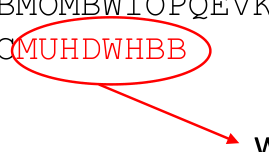
\includegraphics[width=29.40mm,height=41.58mm]{images/llm/page_010_img_02.png}%
\end{textblock*}

\newpage

% --- unit llm 11 ---
% === Halaman 11 (llm) ===

\begin{itemize}
    \item Contoh di dalam Caesar Cipher, misalkan penyerang tahu cipherteks:
    
    KHOOR ZRUOG
    
    dan juga tahu plainteks-nya seharusnya mengandung kata:
    
    HELLO
    
    Dari pasangan $\text{H} \rightarrow \text{K}$, penyerang tahu pergeseran $(k) = 3$.
\end{itemize}

Dengan kunci $k = 3$, semua cipherteks lain bisa didekripsi.

\newpage

% --- unit llm 12 ---
% === Halaman 12 (llm) ===

\section*{3. Chosen-plaintext attack}

Kriptanalis dapat memilih plainteks sesuka hati untuk dienkripsikan, yaitu plainteks-plainteks yang lebih mengarahkan penemuan kunci, lalu mengirim plainteks ke sistem enkripsi. Asumsi: Penyerang memiliki akses ke sistem enkripsi

\vspace{5mm}

Diberikan: \[ P_1, C_1 = E_k(P_1), P_2, C_2 = E_k(P_2), \dots, P_i, C_i = E_k(P_i) \]
di mana kriptanalis dapat memilih diantara $P_1, P_2, \dots, P_i$

Deduksi: $k$ untuk mendapatkan $P_{i+1}$ dari $C_{i+1} = E_k(P_{i+1})$.

\vspace{5mm}

\begin{center}
\textbf{\color{red}Chosen-Plaintext Attack}
\end{center}

\vspace{10mm}

% deskripsi: Diagram ilustrasi serangan Chosen-Plaintext Attack yang melibatkan Alice, Eve (penyerang), dan Bob, menunjukkan bagaimana Eve memilih plainteks, mendapatkan cipherteks, dan menganalisisnya untuk menemukan kunci.
% bbox normalisasi: [0.2700, 0.6600, 0.7400, 0.9600]
\begin{textblock*}{98.70mm}(56.70mm,196.02mm)
\noindent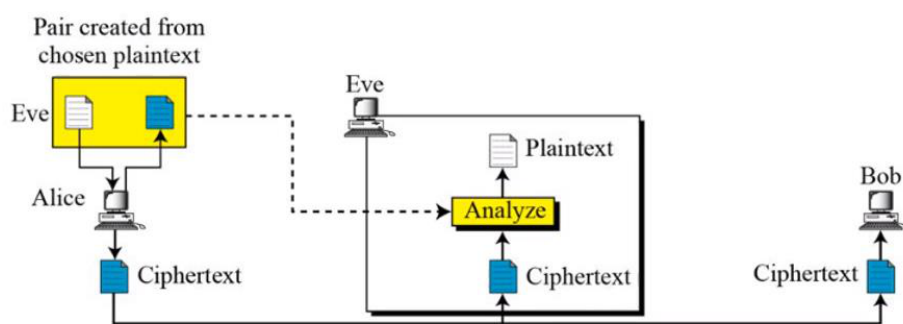
\includegraphics[width=98.70mm,height=89.10mm]{images/llm/page_012_img_01.png}%
\end{textblock*}

\newpage

% --- unit llm 13 ---
% === Halaman 13 (llm) ===

\begin{itemize}
  \item Contoh pada Caesar Cipher, penyerang memilih plainteks sederhana, misalnya:
  
  AAAAA
  
  lalu mengirim plainteks ke sistem enkripsi
  
  Sistem mengembalikan cipherteks, misalnya:
  
  FFFFF
  
  Dari sini terlihat huruf A $\rightarrow$ F, berarti pergeseran = 5.
\end{itemize}

Dengan kunci itu, penyerang bisa mendekripsi semua cipherteks lain.

\newpage

% --- unit llm 14 ---
% === Halaman 14 (llm) ===

\begin{itemize}
    \item Contoh di dalam Vigenere Cipher, cipherteks setiap huruf plainteks dihitung dengan:
    \[ C = (P + K) \pmod{26} \]
    \item Penyerang memilih plaintext P = AAAAAAA... (= 000000...).
    \item Maka cipherteks yang keluar, C, pasti sama dengan K $(C = K)$.
    \item Dengan mengetahui K, cipherteks lain bisa langsung dicoba didekripsi dengan K tersebut.
\end{itemize}

\newpage

% --- unit llm 15 ---
% === Halaman 15 (llm) ===

ATM mengenkripsi PIN dengan kunci $k$ lalu mengirim cipherteks ke komputer di bank

\[ \text{Cipher}(k, PIN) \]

\vspace{20mm}

Kriptanalis ke-1 mengubah PIN lalu memasukkan PIN tsb ke ATM

\vspace{20mm}

Kriptanalis ke-2 menyadap cipherteks dan mempelajarinya untuk mendeduksi kunci $k$

\vspace{10mm}

\begin{center}
\Large \textit{Chosen-plaintext attack}
\end{center}

% deskripsi: Diagram ilustrasi Chosen-plaintext attack yang menunjukkan interaksi antara pengguna/kriptanalis, mesin ATM, bank, dan penyadap (kriptanalis kedua).
% bbox normalisasi: [0.1400, 0.2000, 0.9000, 0.7200]
\begin{textblock*}{159.60mm}(29.40mm,59.40mm)
\noindent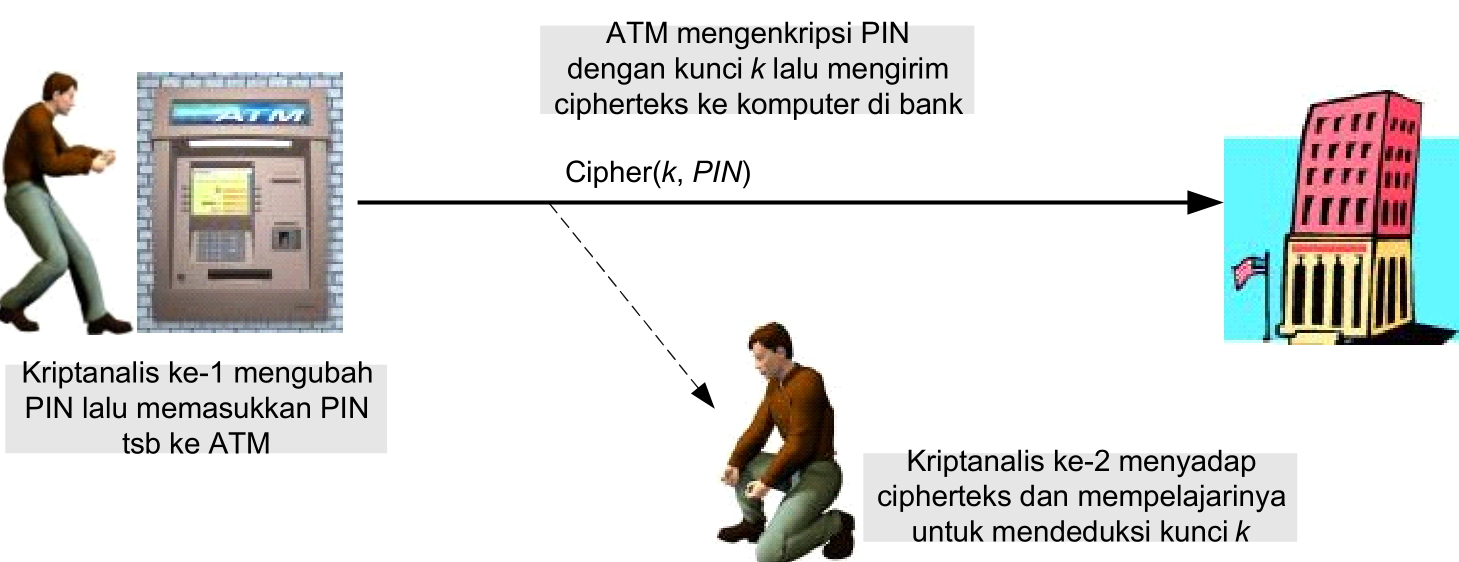
\includegraphics[width=159.60mm,height=154.44mm]{images/llm/page_015_img_01.png}%
\end{textblock*}

\newpage

% --- unit llm 16 ---
% === Halaman 16 (llm) ===

\section*{4. Adaptive-chosen-plaintext attack}

\begin{itemize}
    \item Adaptive chosen plaintext attack adalah variasi dari chosen plaintext attack, dalam hal ini penyerang \textbf{tidak hanya memilih plainteks}, tapi dapat \textbf{menyesuaikan plainteks berikutnya} berdasarkan hasil ciphertext dari query sebelumnya.
    \item Artinya, penyerang belajar secara bertahap: setelah melihat hasil enkripsi pertama, ia memilih plainteks baru yang lebih "cerdas" untuk menggali informasi lebih dalam tentang algoritma/kunci.
\end{itemize}

\newpage

% --- unit llm 17 ---
% === Halaman 17 (llm) ===

\begin{itemize}
    \item Contoh di dalam Caesar Cipher, penyerang memilih plainteks:
    
    A \\ $\rightarrow$ Cipherteks keluar: F. Artinya pergeseran mungkin 5.

    Untuk memastikan, penyerang pilih plainteks lain:
    
    B \\ $\rightarrow$ Cipherteks keluar: G. Polanya konsisten, maka kunci pergeseran dipastikan = 5.
\end{itemize}

\newpage

% --- unit llm 18 ---
% === Halaman 18 (llm) ===

Contoh di dalam Vigenere Cipher:

\begin{itemize}
    \item Enkripsi setiap huruf plainteks:
    \[ C = (P + K) \pmod{26} \]
    \item Penyerang adaptif:
    \begin{itemize}
        \item Pertama masukkan plainteks = AAAA (=0000), maka ciphertext C = K.
        \item Setelah tahu K, ia coba plainteks lain untuk memverifikasi, misalnya BBBB (=1111), hasilnya menegaskan hasil enkripsi dengan K yang sama.
        \item Dengan informasi itu, cipherteks lain bisa langsung dipecahkan.
    \end{itemize}
\end{itemize}

\newpage

% --- unit llm 19 ---
% === Halaman 19 (llm) ===

\section*{5. Chosen-ciphertext attack}

Penyerang dapat memilih cipherteks tertentu dan mendekripsinya dengan oracle yang bisa mendekripsi, dan menggunakan hasil dekripsi untuk memecahkan cipher atau menemukan kunci.

\[ C_1, P_1 = D_k(C_1), C_2, P_2 = D_k(P_2), \dots, C_i, P_i = D_k(C_i) \]

Deduksi: $k$ (yang mungkin diperlukan untuk mendekripsi pesan pada waktu yang akan datang).

\vspace{10mm}

\begin{center}
\color{red} \textbf{Chosen-Ciphertext Attack}
\end{center}

% deskripsi: Diagram alur Chosen-Ciphertext Attack yang melibatkan Alice, Eve, dan Bob, menunjukkan bagaimana Eve memilih ciphertext, mendapatkannya melalui Bob, dan menganalisis plaintext hasilnya.
% bbox normalisasi: [0.3200, 0.7300, 0.7800, 0.9600]
\begin{textblock*}{96.60mm}(67.20mm,216.81mm)
\noindent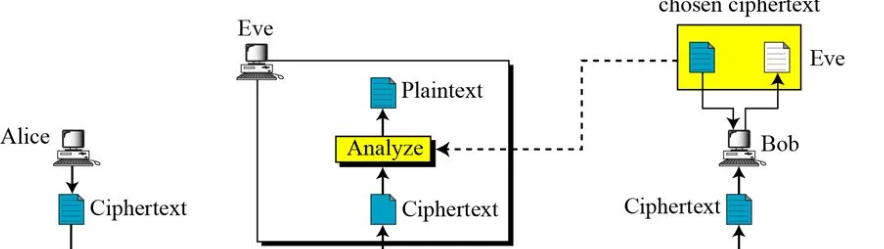
\includegraphics[width=96.60mm,height=68.31mm]{images/llm/page_019_img_01.png}%
\end{textblock*}

\newpage

% --- unit llm 20 ---
% === Halaman 20 (llm) ===

\begin{itemize}
    \item Contoh di dalam Caesar cipher, penyerang memilih cipherteks:
    \[ C = 'A' \]
    lalu sistem dekripsi menghasilkan plainteks:
    \[ P = 'X' \]
    berarti penyerang mengetahui pergeseran huruf $(k) = 3$
\end{itemize}

\newpage

% --- unit llm 21 ---
% === Halaman 21 (llm) ===

Sebuah algoritma kriptografi dikatakan aman secara komputasi (\textit{computationally secure}) bila ia memenuhi tiga kriteria berikut:

\begin{enumerate}
    \item Persamaan matematika yang menggambarkan operasi di dalam algoritma kriptografi sangat kompleks sehingga algoritma tidak mungkin dipecahkan secara analitik.
    \item Biaya untuk memecahkan cipherteks melampaui nilai informasi yang terkandung di dalam cipherteks tersebut.
    \item Waktu yang diperlukan untuk memecahkan cipherteks melampaui lamanya waktu informasi tersebut harus dijaga kerahasiaannya.
\end{enumerate}

\newpage

% --- unit llm 22 ---
% === Halaman 22 (llm) ===

\section*{Jenis-jenis Serangan (2)}

\begin{itemize}
    \item Berdasarkan berdasarkan tujuan atau hasil yang ingin dicapai penyerang:
    \begin{enumerate}
        \item \textit{Key-Recovery Attack}
        \item \textit{Plaintext-Recovery Attack}
        \item \textit{Distinguishing Attack}
        \item \textit{Forgery Attack}
        \item \textit{Replay Attack}
    \end{enumerate}
\end{itemize}

\newpage

% --- unit llm 23 ---
% === Halaman 23 (llm) ===

\section*{1. Key-Recovery Attack}

\begin{itemize}
    \item Tujuan: memperoleh kunci kriptografi yang digunakan untuk mengenkripsi/dekripsi.
    \item Misalkan sebuah sistem menggunakan
    \[ C = E_K(P) \quad , \quad P = \text{plainteks}, \ K = \text{kunci}, \ C = \text{cipherteks} \]
    \item Dalam \textit{key-recovery attack}, penyerang berusaha menemukan K.
    \item Contoh: Misalkan sebuah cipher menggunakan kunci 16 karakter. Penyerang melakukan pencarian kunci secara \textit{brute force}:
    
    \begin{align*}
    K_1 & \to \text{dekripsi } C \to P_1 \\
    K_2 & \to \text{dekripsi } C \to P_2 \\
    K_3 & \to \text{dekripsi } C \to P_3 \\
    & \vdots
    \end{align*}
    sampai ditemukan kunci yang menghasilkan plainteks yang masuk akal.
\end{itemize}

\newpage

% --- unit llm 24 ---
% === Halaman 24 (llm) ===

\section*{2. Plaintext-Recovery Attack}

\begin{itemize}
    \item Tujuan: memperoleh plainteks, tetapi tidak harus memperoleh kunci.
    \item Contoh: Misalkan sebuah cipherteks dikirimir:
    \[ C = XQZ\dots \]
    Penyerang menganalisis struktur cipherteks dan mengetahui bahwa pesan tersebut kemungkinan berbunyi:
    \[ \text{MEET AT THE STATION} \]
    tanpa mengetahui kunci sebenarnya.
\end{itemize}

Dalam beberapa situasi, mendapatkan plainteks tertentu sudah cukup bagi penyerang. Misalnya, jika pesan berisi informasi penting, penyerang mungkin tidak perlu mengetahui kunci untuk mencapai tujuannya.

\newpage

% --- unit llm 25 ---
% === Halaman 25 (llm) ===

\section*{3. Distinguishing Attack}

\begin{itemize}
    \item Tujuan: menentukan apakah suatu data merupakan keluaran algoritma kriptografi atau data yang benar-benar acak (random).
    \item Jika secara statistik penyerang dapat membedakannya dengan probabilitas yang secara signifikan lebih baik daripada tebakan acak, berarti terdapat \textit{distinguishing attack}.
    \vspace{5mm}
    \item Contoh: misalkan sebuah cipher menghasilkan:
    \[ 10101010101010101010101010... \]
    Pola tersebut jelas tidak menyerupai random.
    Penyerang dapat membuat distinguisher sederhana:
    \textit{Jika jumlah 0 dan 1 sangat tidak seimbang atau terdapat pola tertentu, kemungkinan data tersebut berasal dari cipher.}
    \vspace{5mm}
    \item \textit{Cipher} modern dirancang agar kelemahan seperti ini tidak mudah ditemukan.
\end{itemize}

\newpage

% --- unit llm 26 ---
% === Halaman 26 (llm) ===

\section*{4. Forgery Attack}

\begin{itemize}
    \item Tujuan: membuat pesan palsu yang diterima sebagai pesan sah oleh sistem.
    \item Serangan ini sangat penting pada sistem yang menggunakan MAC (\textit{message authentication code}) atau \textit{digital signature} (akan dijelaskan pada materi kuliah selanjutnya).
    \item Misalkan Alice mengirim Pesan + MAC kepada Bob.
    \item Bob memeriksa MAC untuk memastikan pesan benar-benar berasal dari pihak yang memiliki kunci.
    \item Penyerang, Eve, ingin membuat:
    
    Pesan palsu + MAC yang valid
    
    sehingga Bob menganggap pesan tersebut autentik.
\end{itemize}

\newpage

% --- unit llm 27 ---
% === Halaman 27 (llm) ===

\section*{5. Replay Attack}

\begin{itemize}
    \item Tujuan: menggunakan kembali pesan sah yang pernah dikirim sebelumnya untuk menyebabkan suatu tindakan terjadi lagi.
    \item Yang menarik, pada \textit{replay attack} penyerang tidak perlu memecahkan enkripsi.
    \item Untuk mencegah \textit{replay attack}, biasanya digunakan mekanisme yang membuat setiap pesan mempunyai keunikan atau urutan, misalnya: \textit{Nonce, Timestamp}, atau \textit{Sequence number}
    \item Misalnya pesan diberi \textit{sequence number}:
    
    Message 101 \\
    Message 102 \\
    Message 103
    
    Jika penyerang mengirim kembali Message 101 setelah sistem sudah menerima Message 103, sistem dapat menolaknya karena nomor tersebut sudah kedaluwarsa.
\end{itemize}

\newpage

% --- unit llm 28 ---
% === Halaman 28 (llm) ===

Sumber: William Stalling, Cryptography and Network Security
Overview & Chapter 1

\vspace{60mm}

\begin{center}
\Large \textbf{Replay Attack}
\end{center}

% deskripsi: Ilustrasi serangan replay attack yang melibatkan Bob (pengirim), Alice (penerima), dan Darth (penyerang) yang mencegat pesan melalui Internet atau fasilitas komunikasi lainnya untuk kemudian dikirim ulang kepada Alice.
% bbox normalisasi: [0.1800, 0.2200, 0.8200, 0.7800]
\begin{textblock*}{134.40mm}(37.80mm,65.34mm)
\noindent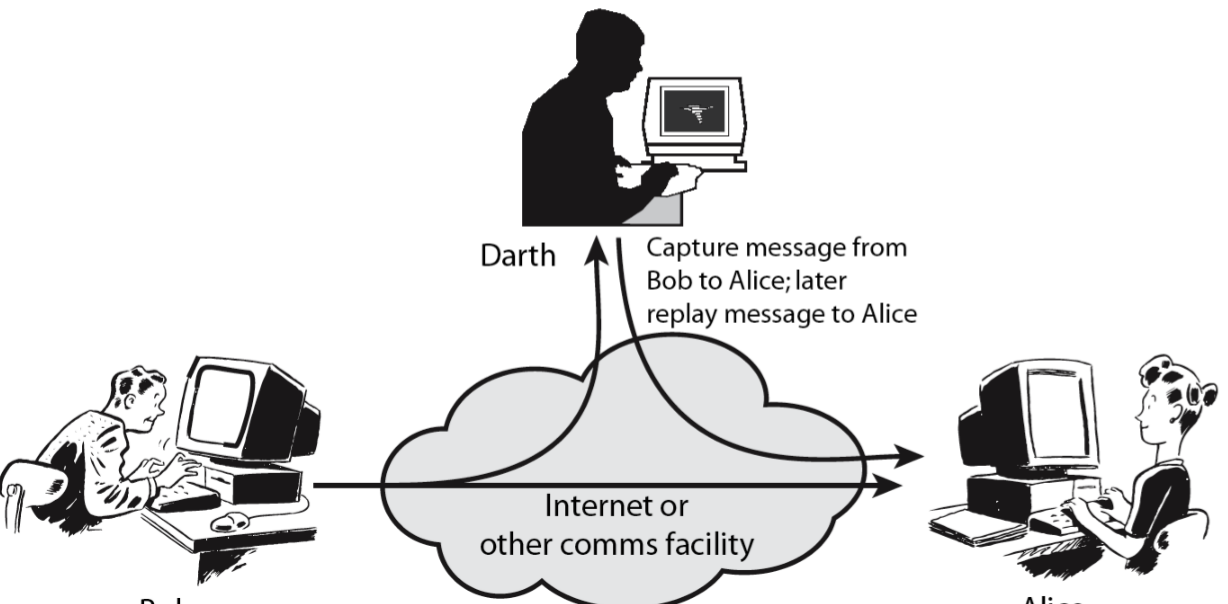
\includegraphics[width=134.40mm,height=166.32mm]{images/llm/page_028_img_01.png}%
\end{textblock*}

\newpage

% --- unit llm 29 ---
% === Halaman 29 (llm) ===

\section*{Jenis-jenis Serangan (3)}

Berdasarkan keterlibatan penyerang dalam komunikasi pesan:
\begin{enumerate}
    \item Serangan pasif
    \item Serangan aktif
\end{enumerate}

\newpage

% --- unit llm 30 ---
% === Halaman 30 (llm) ===

\section*{1. Serangan pasif (passive attack)}

\begin{itemize}
    \item penyerang tidak terlibat dalam komunikasi antara pengirim dan penerima
    \item penyerang hanya melakukan penyadapan untuk memperoleh data atau informasi sebanyak-banyaknya
    \item enkripsi pesan mencegah penyadap memahami isi pesan
\end{itemize}

\vspace{10mm}

% deskripsi: Ilustrasi serangan pasif yang menunjukkan Alice mengirim pesan terenkripsi kepada Bob, sementara Eve bertindak sebagai penyadap (eavesdropper) yang mencoba mengintip komunikasi tersebut.
% bbox normalisasi: [0.2060, 0.5060, 0.8230, 0.8830]
\begin{textblock*}{129.57mm}(43.26mm,150.28mm)
\noindent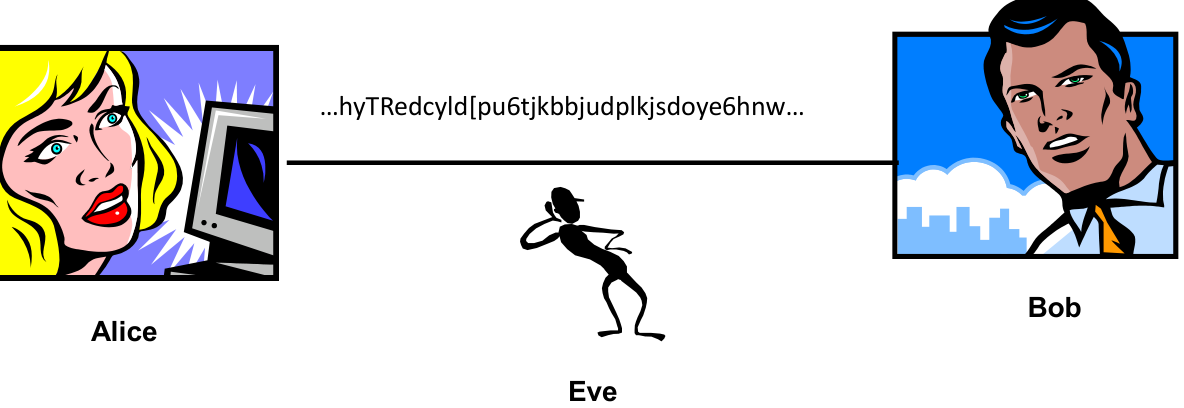
\includegraphics[width=129.57mm,height=111.97mm]{images/llm/page_030_img_01.png}%
\end{textblock*}

\newpage

% --- unit llm 31 ---
% === Halaman 31 (llm) ===

Sumber: William Stalling, Cryptography and Network Security\nOverview & Chapter 1

\vspace{60mm}

\begin{center}
\textbf{Passive Attack : Interception}
\end{center}

% deskripsi: Diagram ilustrasi serangan pasif berupa intersep pesan antara Bob dan Alice melalui Internet, di mana pihak ketiga bernama Darth menyadap konten pesan.
% bbox normalisasi: [0.1500, 0.1900, 0.7900, 0.7700]
\begin{textblock*}{134.40mm}(31.50mm,56.43mm)
\noindent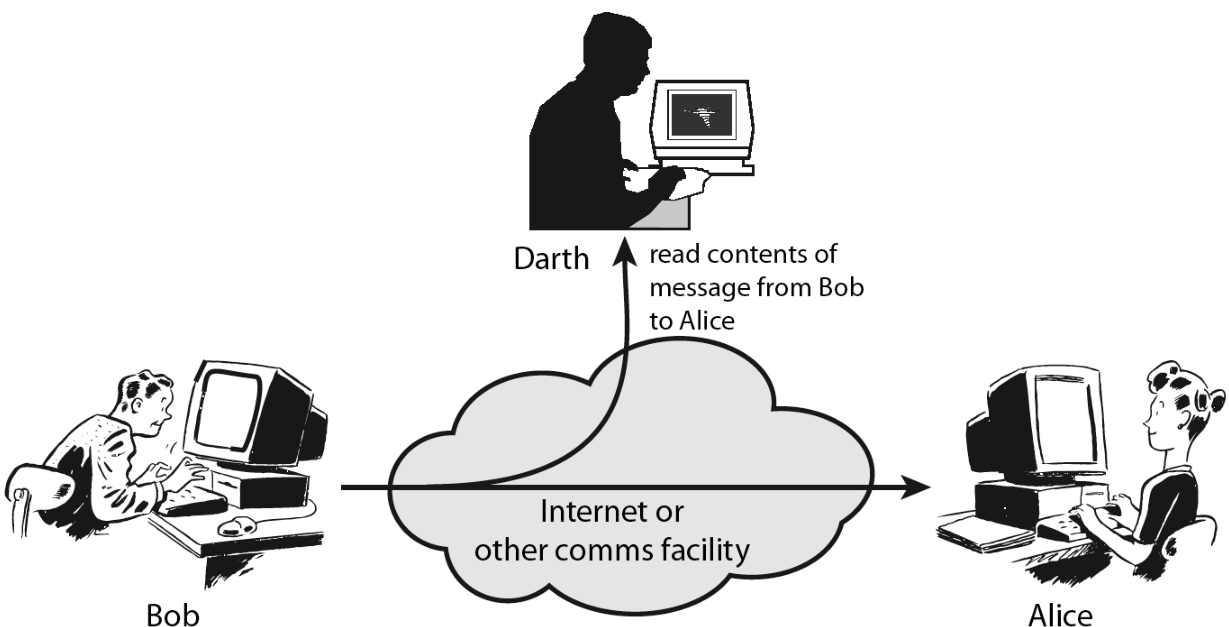
\includegraphics[width=134.40mm,height=172.26mm]{images/llm/page_031_img_01.png}%
\end{textblock*}

\newpage

% --- unit llm 32 ---
% === Halaman 32 (llm) ===

\vspace{172.26mm}

Sumber: William Stalling, Cryptography and Network Security
Overview & Chapter 1

\vspace{60mm}

\textbf{Passive Attack : Traffic Analysis}

% deskripsi: Diagram yang mengilustrasikan analisis lalu lintas (traffic analysis) sebagai serangan pasif, menampilkan Bob dan Alice yang berkomunikasi melalui Internet atau fasilitas komunikasi lainnya, sementara penyerang bernama Darth mengamati pola lalu lintas data tersebut.
% bbox normalisasi: [0.1400, 0.1400, 0.7800, 0.7200]
\begin{textblock*}{134.40mm}(29.40mm,41.58mm)
\noindent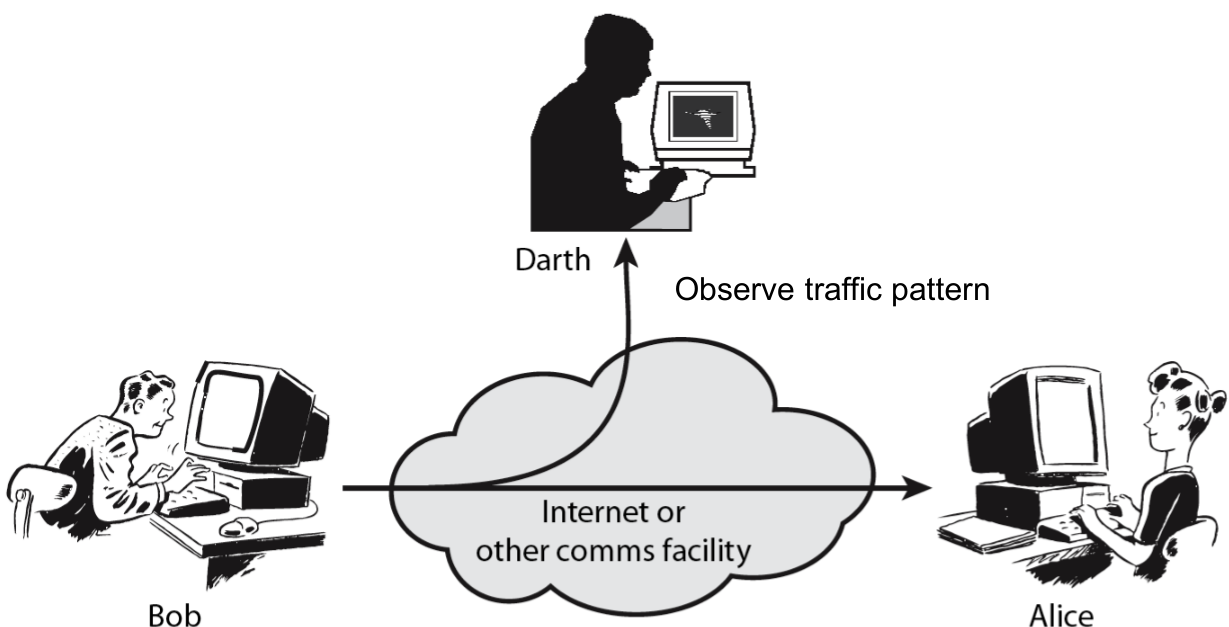
\includegraphics[width=134.40mm,height=172.26mm]{images/llm/page_032_img_01.png}%
\end{textblock*}

\newpage

% --- unit llm 33 ---
% === Halaman 33 (llm) ===

\vspace{227.50mm}

\begin{center}
\Huge Screenshot Wireshark (memantau network traffic)
\end{center}

\vspace{10mm}

% deskripsi: Screenshot aplikasi Wireshark yang menampilkan penangkapan paket data jaringan dari Marvell Yukon Ethernet Controller, mencakup daftar paket dengan kolom No, Time, Source, Destination, Protocol, Length, dan Info, serta panel detail paket dalam bentuk heksadesimal dan teks.
% bbox normalisasi: [0.1510, 0.1570, 0.8020, 0.9230]
\begin{textblock*}{136.71mm}(31.71mm,46.63mm)
\noindent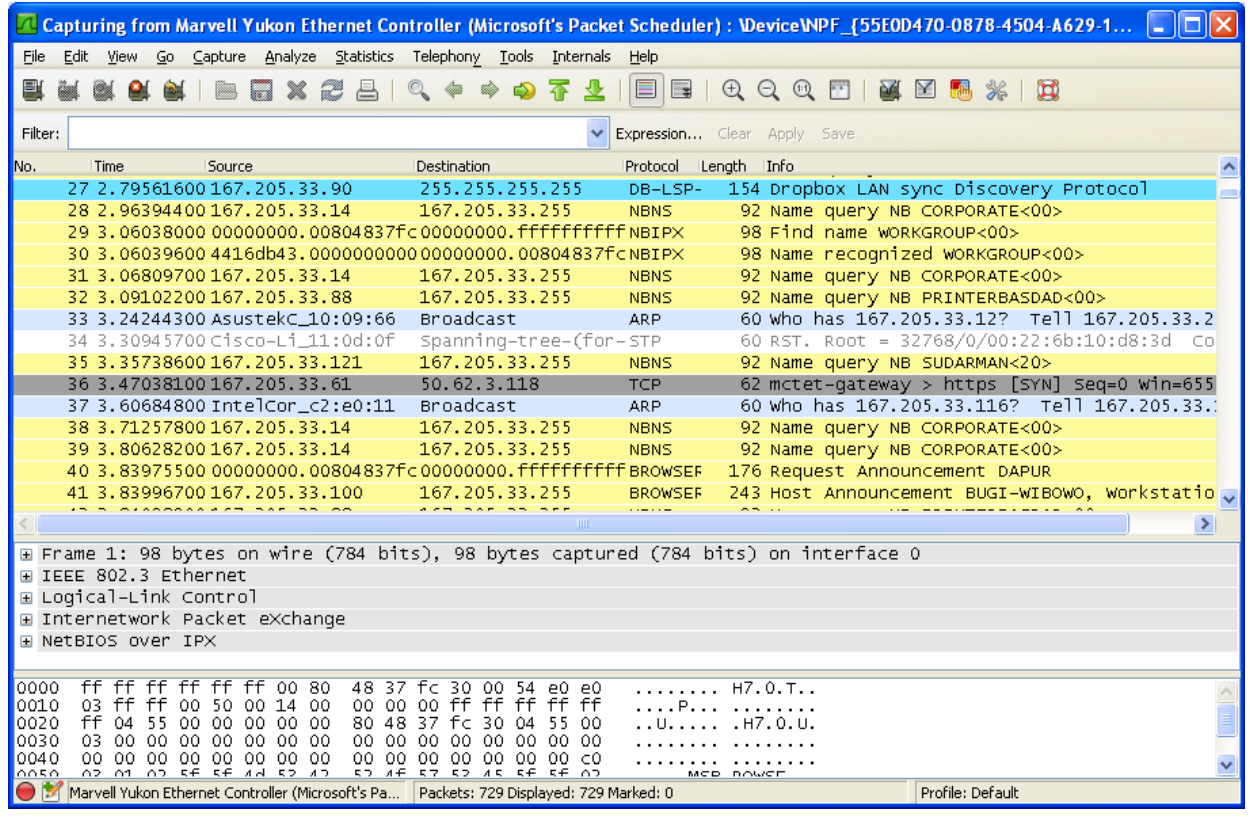
\includegraphics[width=136.71mm,height=227.50mm]{images/llm/page_033_img_01.png}%
\end{textblock*}

\newpage

% --- unit llm 34 ---
% === Halaman 34 (llm) ===

Filtering dengan penerapan Wireshark dapat menampilkan plainteks berupa username dan password\vspace{10mm}

\vspace{115.83mm}

Sumber gambar: https://www.researchgate.net/figure/Wireshark-Filtering-Showing-Clear-Text-of-user-Name-and-Password\_fig3\_326419957

% deskripsi: Screenshot aplikasi Wireshark yang menunjukkan proses analisis paket HTTP POST, memperlihatkan data form yang tidak terenkripsi berisi username 'Ibrahim\_Diyeb' dan password 'yemen\_123'.
% bbox normalisasi: [0.1050, 0.3300, 0.8450, 0.7200]
\begin{textblock*}{155.40mm}(22.05mm,98.01mm)
\noindent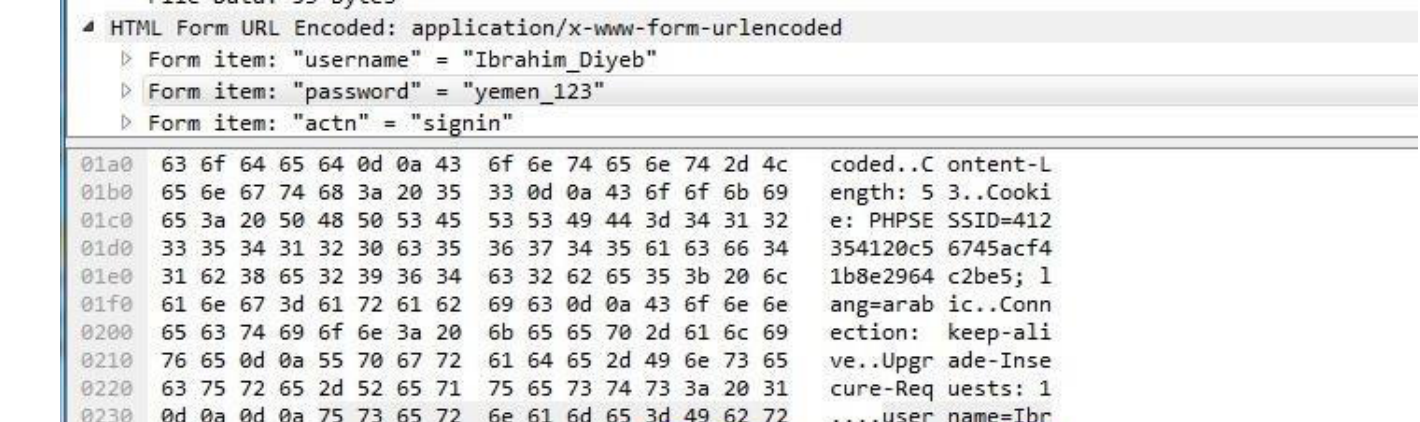
\includegraphics[width=155.40mm,height=115.83mm]{images/llm/page_034_img_01.png}%
\end{textblock*}

\newpage

% --- unit llm 35 ---
% === Halaman 35 (llm) ===

Cek video TUTORIAL CARA MENGGUNAKAN WIRESHARK | MENEMUKAN U53RN4M3 P455WORD PADA LALU LINTAS PACKET JARINGAN:\newline\url{https://www.youtube.com/watch?v=HMkIhUEByd4}

\vspace{70mm}

TUTORIAL CARA MENGGUNAKAN WIRESHARK | MENEMUKAN U53RN4M3 P455WORD PADA LALU LINTAS PACKET JARINGAN

% deskripsi: Screenshot tampilan layar browser yang menampilkan video tutorial YouTube mengenai penggunaan Wireshark untuk memonitoring jaringan dan analisis paket data.
% bbox normalisasi: [0.1400, 0.2100, 0.7400, 0.8900]
\begin{textblock*}{126.00mm}(29.40mm,62.37mm)
\noindent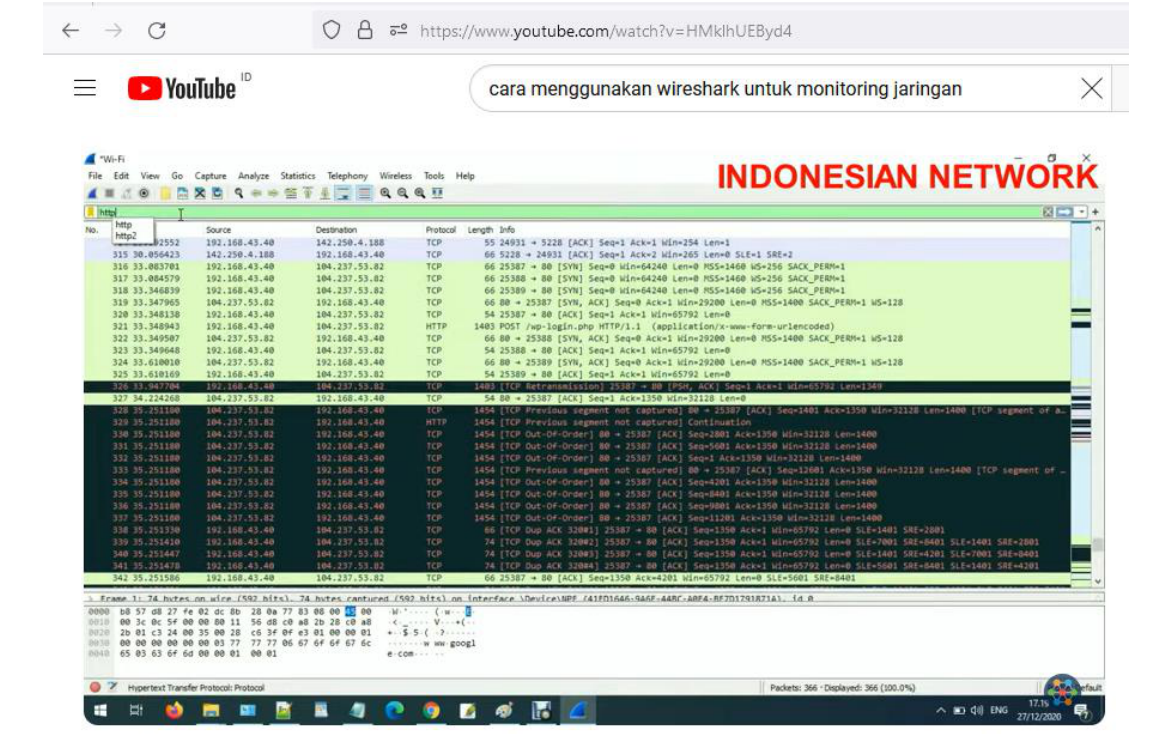
\includegraphics[width=126.00mm,height=201.96mm]{images/llm/page_035_img_01.png}%
\end{textblock*}

\newpage

% --- unit llm 36 ---
% === Halaman 36 (llm) ===

\textbf{Metode penyadapan:}
\begin{enumerate}
  \item Wiretapping
  \item Electromagnetic eavesdropping
  \item Acoustic Eavesdropping
\end{enumerate}

\newpage

% --- unit llm 37 ---
% === Halaman 37 (llm) ===

\begin{itemize}
    \item \textbf{Wiretapping}
\end{itemize}

\vspace{60mm}

Baca di sini:
\begin{enumerate}
    \item \url{https://hackaday.com/2008/06/19/wiretapping-and-how-to-avoid-it/}
    \item \url{https://edition.cnn.com/videos/us/2017/03/07/what-is-wiretapping-jpm-orig.cnn}
\end{enumerate}

% deskripsi: Diagram ilustrasi cara kerja penyadapan telepon (simple line tap) yang menunjukkan koneksi antara power supply, alat wiretap, dan telepon.
% bbox normalisasi: [0.2180, 0.1840, 0.8570, 0.7340]
\begin{textblock*}{134.19mm}(45.78mm,54.65mm)
\noindent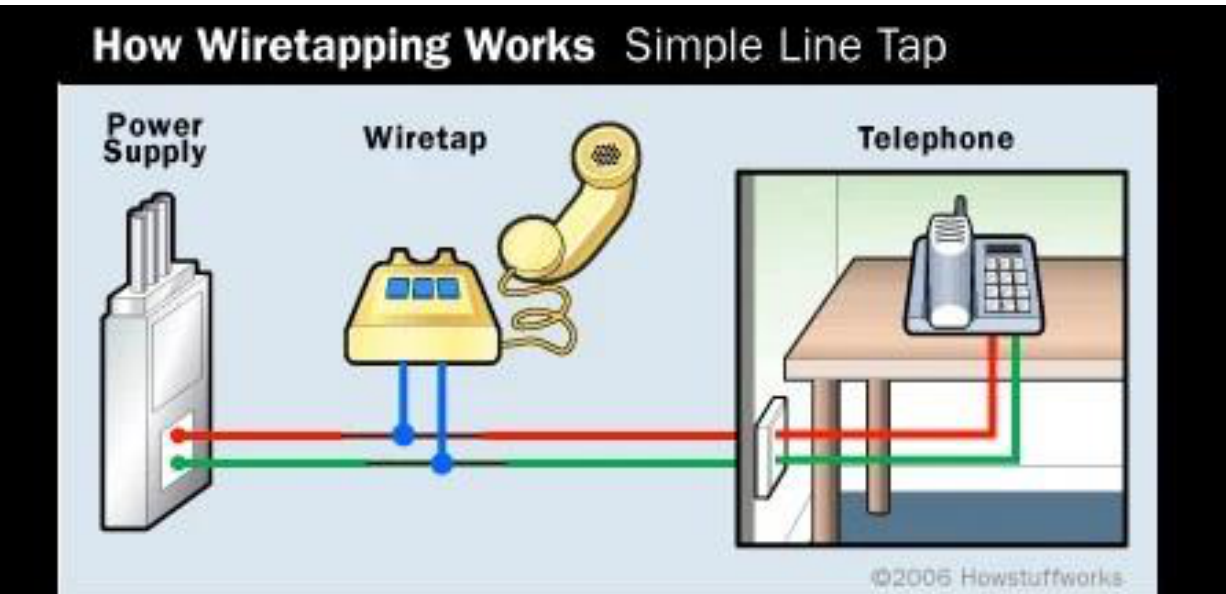
\includegraphics[width=134.19mm,height=163.35mm]{images/llm/page_037_img_01.png}%
\end{textblock*}

\newpage

% --- unit llm 38 ---
% === Halaman 38 (llm) ===

\section*{How Wiretapping Works}
(sumber: http://www.howstuffworks.com/wiretapping.htm)

\vspace{60mm}

When you open up a phone, you can see that the technology inside is very simple. The simplicity of design makes the phone system vulnerable to surreptitious eavesdropping.

\vspace{10mm}

Inside a standard phone cord, you'll find a red wire and a green wire. These wires form a circuit like the one you might find in a flashlight. Just as in a flashlight, there is a negatively-charged end and a positively-charged end to the circuit. In a telephone cord, the green wire connects to the positive end and the red cord connects to the negative end.

% deskripsi: Foto bagian dalam telepon genggam lama yang memperlihatkan kabel-kabel sederhana.
% bbox normalisasi: [0.1170, 0.2370, 0.4850, 0.7320]
\begin{textblock*}{77.28mm}(24.57mm,70.39mm)
\noindent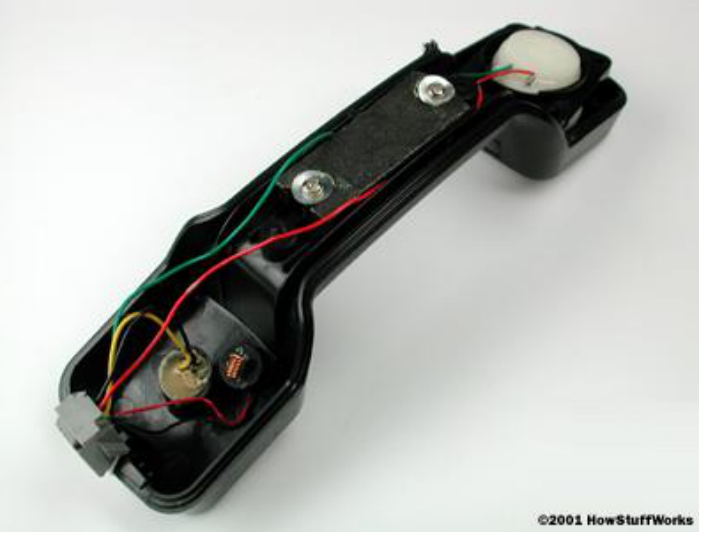
\includegraphics[width=77.28mm,height=147.01mm]{images/llm/page_038_img_01.png}%
\end{textblock*}

% deskripsi: Foto kabel telepon yang dikupas ujungnya, memperlihatkan kabel merah dan hijau.
% bbox normalisasi: [0.5140, 0.2370, 0.9230, 0.6540]
\begin{textblock*}{85.89mm}(107.94mm,70.39mm)
\noindent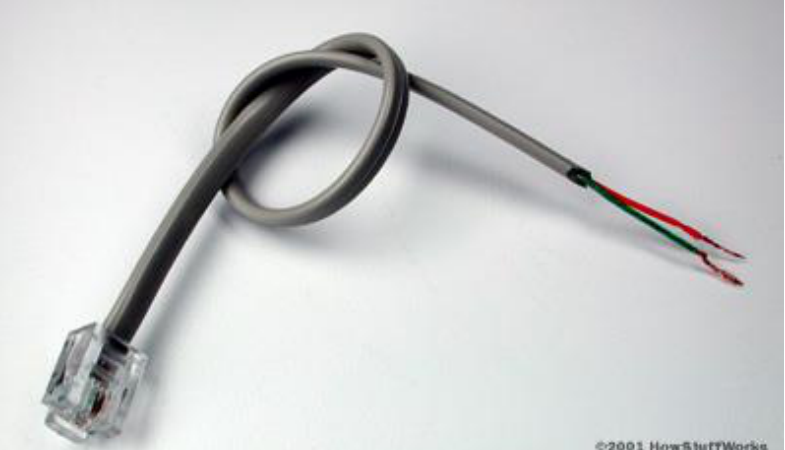
\includegraphics[width=85.89mm,height=123.85mm]{images/llm/page_038_img_02.png}%
\end{textblock*}

\newpage

% --- unit llm 39 ---
% === Halaman 39 (llm) ===

\vspace{172.26mm}

\section*{Electromagnetic eavesdropping}

\vspace{50mm}

Sumber: \url{https://www.researchgate.net/figure/An-anechoic-chamber-Figure-4-Example-for-an-electromagnetic-eavesdropping-process_fig3_324680618}

% deskripsi: Ilustrasi konsep eavesdropping elektromagnetik yang menunjukkan seseorang di satu kantor menggunakan antena penerima untuk menangkap sinyal dari perangkat elektronik (komputer) di kantor sebelah melalui dinding, dengan keterangan jarak r < 2m.
% bbox normalisasi: [0.1300, 0.1600, 0.7800, 0.7400]
\begin{textblock*}{136.50mm}(27.30mm,47.52mm)
\noindent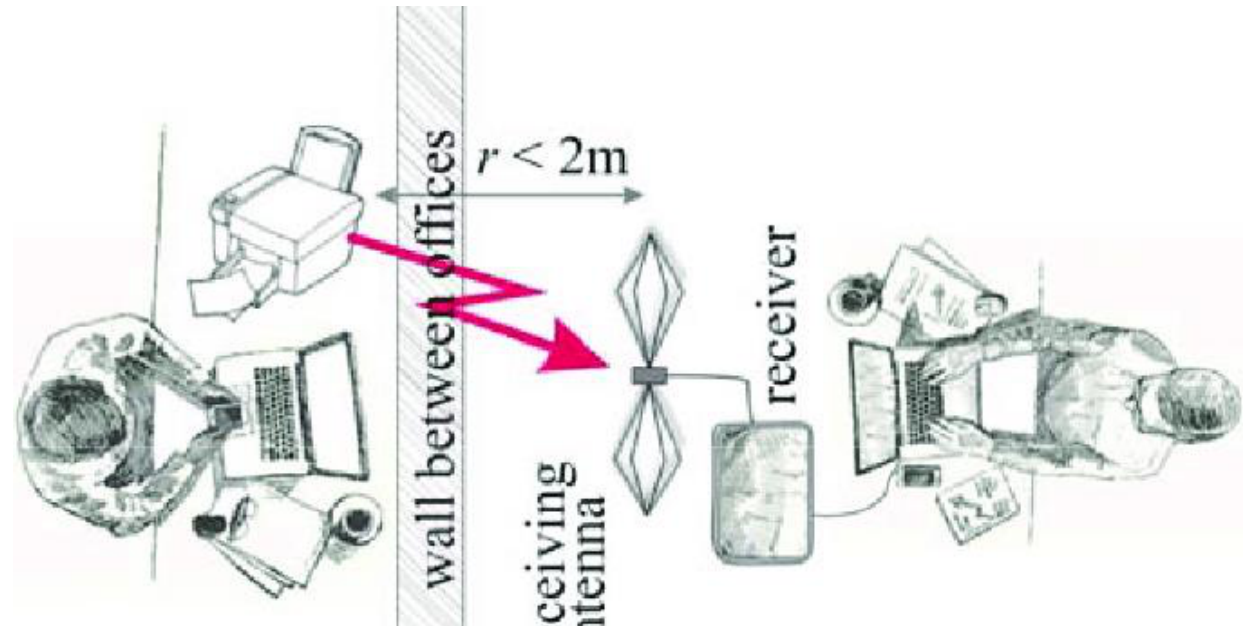
\includegraphics[width=136.50mm,height=172.26mm]{images/llm/page_039_img_01.png}%
\end{textblock*}

\newpage

% --- unit llm 40 ---
% === Halaman 40 (llm) ===

\vspace{222.16mm}

Cek video \textbf{INTERCEPT ANY RADIO SIGNAL!!!!}: \url{https://www.youtube.com/watch?v=UMu5AhSg-TI}

% deskripsi: Screenshot cuplikan video YouTube yang menunjukkan seseorang memegang perangkat penerima sinyal radio (SDR) dengan tampilan spektrogram.
% bbox normalisasi: [0.0960, 0.1770, 0.6980, 0.9250]
\begin{textblock*}{126.42mm}(20.16mm,52.57mm)
\noindent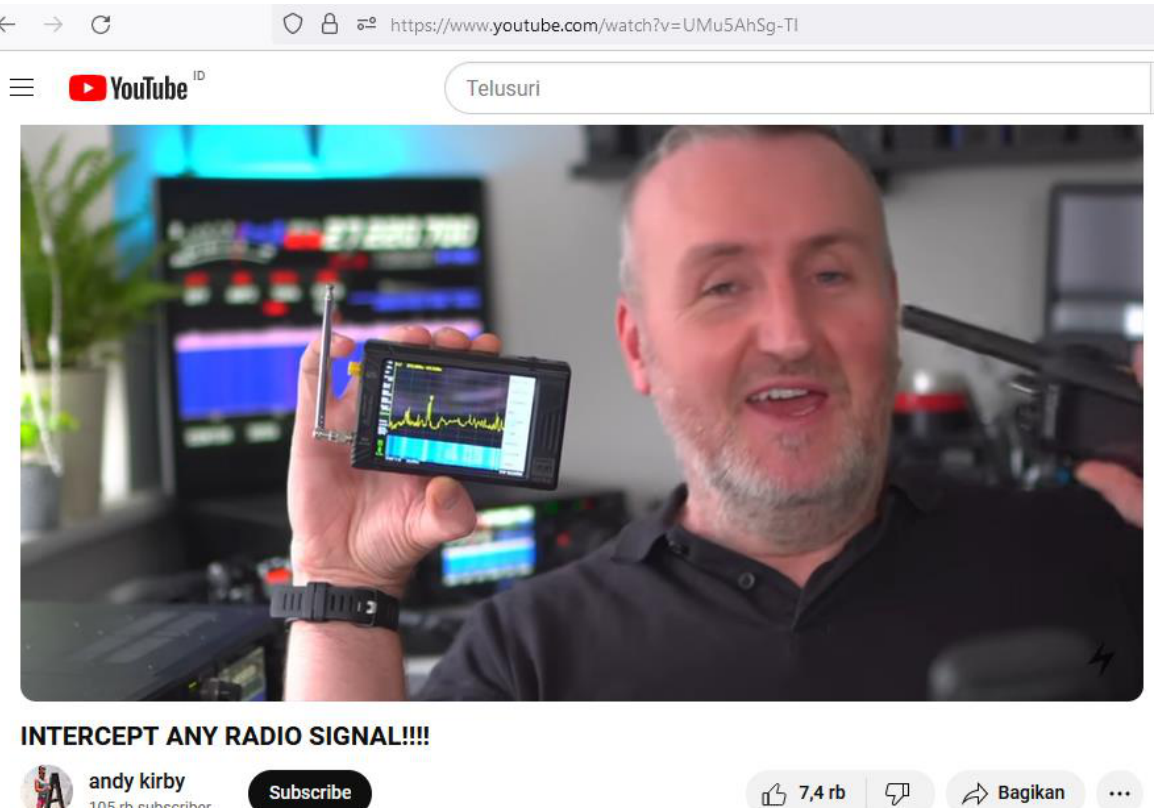
\includegraphics[width=126.42mm,height=222.16mm]{images/llm/page_040_img_01.png}%
\end{textblock*}

\newpage

% --- unit llm 41 ---
% === Halaman 41 (llm) ===

\vspace{210.87mm}

Cek video GSM Sniffing: Voice Decryption 101 - Software Defined Radio Series \#11:\
\url{https://www.youtube.com/watch?v=krJKKjYdwgc}

\vspace{10mm}

GSM Sniffing: Voice Decryption 101 - Software Defined Radio Series \#11

% deskripsi: Screenshot video YouTube yang menampilkan perangkat lunak analisis sinyal radio (SDR) dan terminal command line untuk proses GSM sniffing.
% bbox normalisasi: [0.1500, 0.1500, 0.7500, 0.8600]
\begin{textblock*}{126.00mm}(31.50mm,44.55mm)
\noindent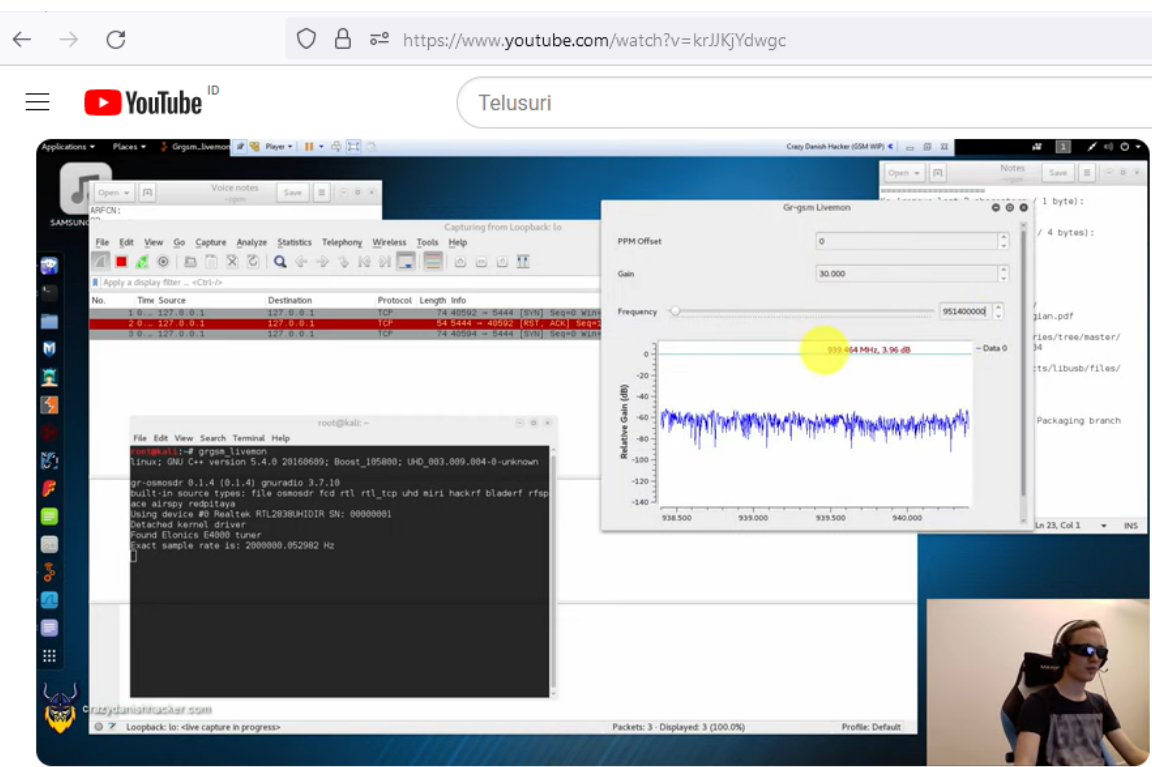
\includegraphics[width=126.00mm,height=210.87mm]{images/llm/page_041_img_01.png}%
\end{textblock*}

\newpage

% --- unit llm 42 ---
% === Halaman 42 (llm) ===

\vspace{146.72mm}

\section*{Acoustic Eavesdropping}

\vspace{10mm}

% deskripsi: Ilustrasi seseorang yang bersembunyi di bawah meja untuk mendengarkan percakapan menggunakan alat perekam dan mikrofon.
% bbox normalisasi: [0.1480, 0.2470, 0.4080, 0.8330]
\begin{textblock*}{54.60mm}(31.08mm,73.36mm)
\noindent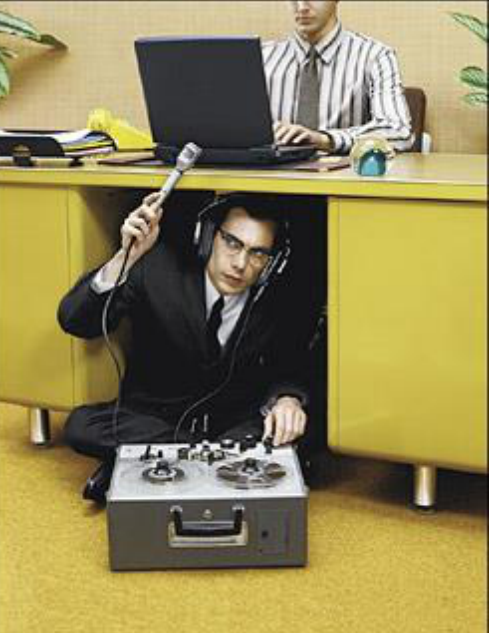
\includegraphics[width=54.60mm,height=174.04mm]{images/llm/page_042_img_01.png}%
\end{textblock*}

% deskripsi: Ilustrasi seseorang yang bersembunyi di bawah meja kantor sementara orang lain sedang berbicara di telepon di atas meja.
% bbox normalisasi: [0.4650, 0.2470, 0.8840, 0.7410]
\begin{textblock*}{87.99mm}(97.65mm,73.36mm)
\noindent
\includegraphics[width=87.99mm,height=146.72mm]{images/llm/page_042_img_02.png}%
\end{textblock*}

\newpage

% --- unit llm 43 ---
% === Halaman 43 (llm) ===

\vspace{178.20mm}

Sumber: \url{https://www.semanticscholar.org/paper/Acoustic-Eavesdropping-through-Wireless-Vibrometry-Wei-Wang/8afd80726c54ed7b95d30d1230bef633d128c930}

% deskripsi: Ilustrasi dua skenario penyadapan akustik: (kiri) metode Reflective menggunakan pengirim (Tx) dan penerima (Rx) untuk mendeteksi getaran dari speaker korban, dan (kanan) metode Emissive menggunakan AP dan penerima (Rx) untuk mendeteksi emisi dari smartphone korban melalui dinding.
% bbox normalisasi: [0.1500, 0.1400, 0.8400, 0.7400]
\begin{textblock*}{144.90mm}(31.50mm,41.58mm)
\noindent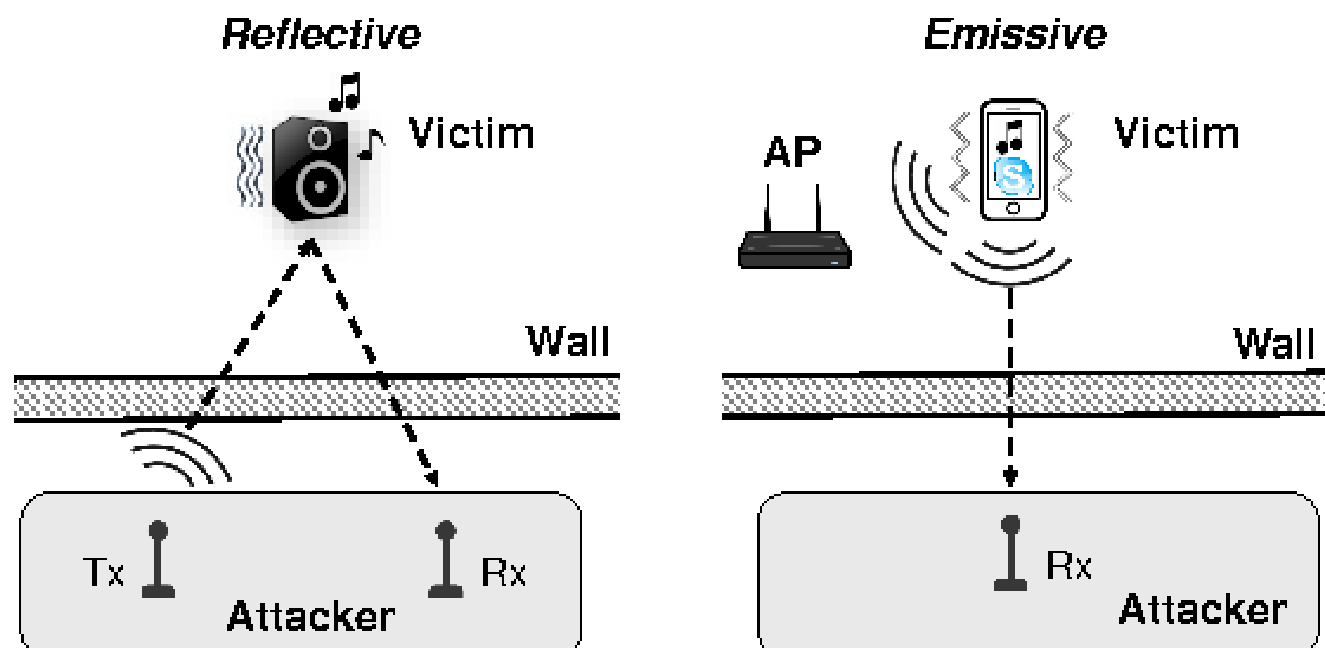
\includegraphics[width=144.90mm,height=178.20mm]{images/llm/page_043_img_01.png}%
\end{textblock*}

\newpage

% --- unit llm 44 ---
% === Halaman 44 (llm) ===

\section*{2. Serangan aktif (active attack)}

\begin{itemize}
    \item penyerang mengintervensi komunikasi dan ikut mempengaruhi sistem untuk keuntungan dirinya
    \item penyerang dapat mengubah aliran pesan seperti:
    \begin{itemize}
        \item menghapus sebagian cipherteks,
        \item mengubah cipherteks,
        \item menyisipkan potongan cipherteks palsu,
        \item me-replay pesan lama,
        \item mengubah informasi yang tersimpan, dsb
    \end{itemize}
    \item Contoh: \textit{man-in-the-middle attack}
\end{itemize}

\newpage

% --- unit llm 45 ---
% === Halaman 45 (llm) ===

\vspace{170.48mm}

Sumber: William Stalling, Cryptography and Network Security\nOverview \& Chapter 1\n\vspace{60mm}
\begin{center}
\textbf{Active Attack: Interruption}
\end{center}

% deskripsi: Diagram ilustrasi serangan aktif berupa gangguan (Interruption), yang menunjukkan Bob mencoba mengirim pesan kepada Alice melalui Internet, namun pengiriman tersebut diblokir oleh penyerang bernama Darth.
% bbox normalisasi: [0.1780, 0.2220, 0.8230, 0.7960]
\begin{textblock*}{135.45mm}(37.38mm,65.93mm)
\noindent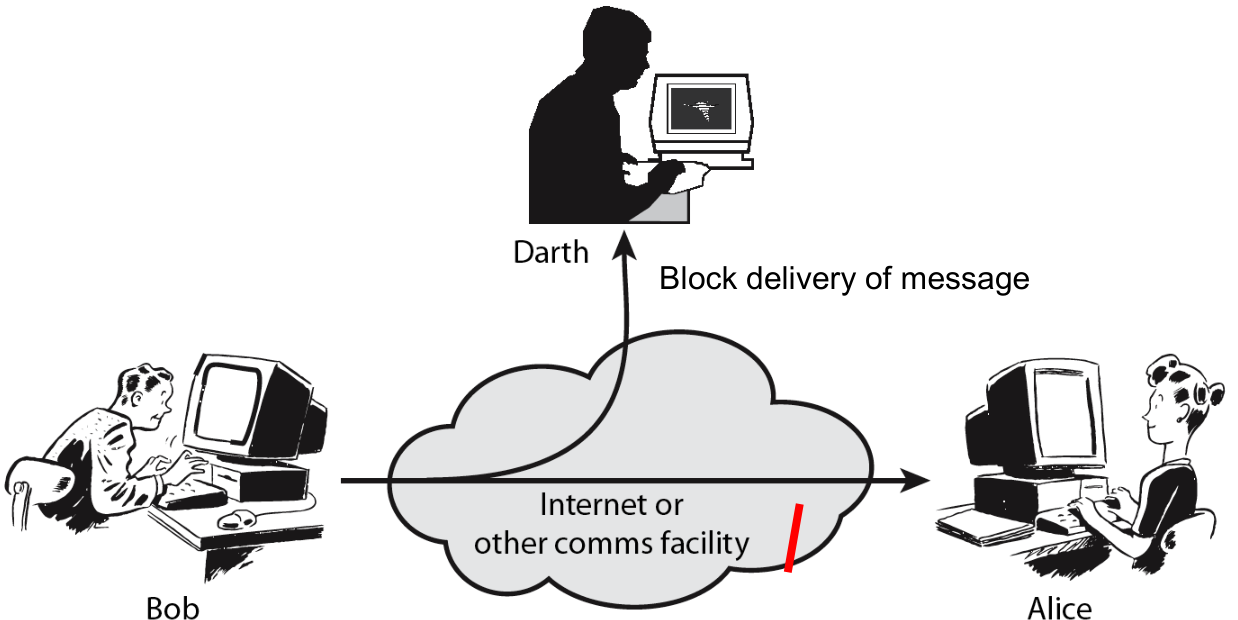
\includegraphics[width=135.45mm,height=170.48mm]{images/llm/page_045_img_01.png}%
\end{textblock*}

\newpage

% --- unit llm 46 ---
% === Halaman 46 (llm) ===

\vspace{175.23mm}

Sumber: William Stalling, Cryptography and Network Security\nOverview & Chapter 1\n\vspace{60mm}\n\textbf{\Large Active Attack: Fabrication}

% deskripsi: Diagram ilustrasi serangan aktif berupa fabrikasi pesan, menunjukkan penyerang (Darth) yang mengirimkan pesan palsu ke Alice melalui internet, menginterupsi komunikasi antara Bob dan Alice.
% bbox normalisasi: [0.1900, 0.1700, 0.8300, 0.7600]
\begin{textblock*}{134.40mm}(39.90mm,50.49mm)
\noindent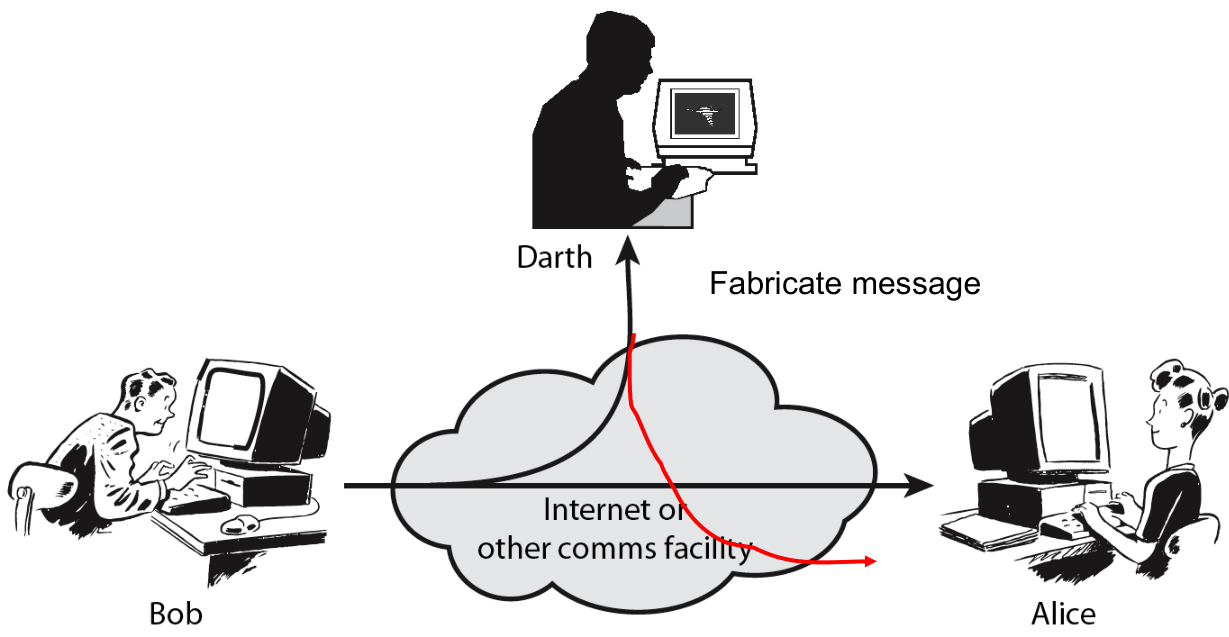
\includegraphics[width=134.40mm,height=175.23mm]{images/llm/page_046_img_01.png}%
\end{textblock*}

\newpage

% --- unit llm 47 ---
% === Halaman 47 (llm) ===

Sumber: William Stalling, Cryptography and Network Security
Overview \& Chapter 1

\vspace{60mm}

\begin{center}
\textbf{\huge Active Attack: Replay}
\end{center}

% deskripsi: Ilustrasi serangan replay yang melibatkan Bob sebagai pengirim, Alice sebagai penerima, dan Darth sebagai penyerang yang menangkap serta mengirim ulang pesan melalui jaringan internet.
% bbox normalisasi: [0.1780, 0.2180, 0.8220, 0.7900]
\begin{textblock*}{135.24mm}(37.38mm,64.75mm)
\noindent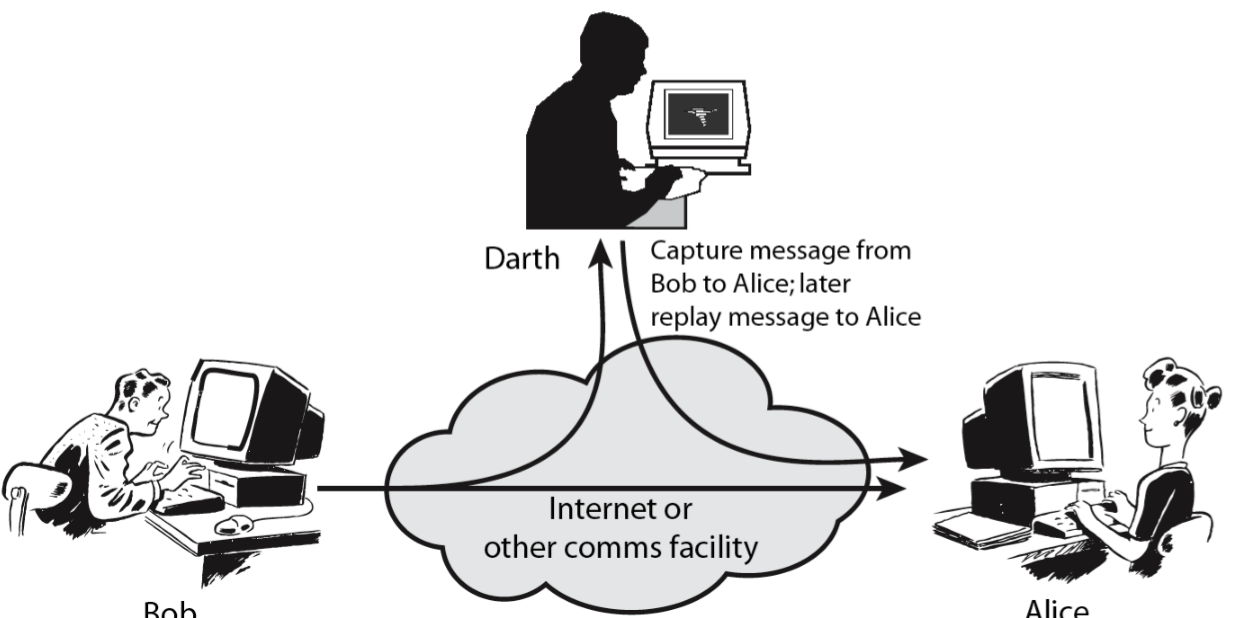
\includegraphics[width=135.24mm,height=169.88mm]{images/llm/page_047_img_01.png}%
\end{textblock*}

\newpage

% --- unit llm 48 ---
% === Halaman 48 (llm) ===

\vspace{172.26mm}

Sumber: William Stalling, Cryptography and Network Security\nOverview & Chapter 1

\vspace{60mm}

\begin{center}
\textbf{Active Attack: Modification}
\end{center}

% deskripsi: Diagram yang mengilustrasikan serangan aktif berupa modifikasi pesan, di mana penyerang bernama Darth mencegat dan mengubah pesan yang dikirim oleh Bob kepada Alice melalui internet atau fasilitas komunikasi lainnya.
% bbox normalisasi: [0.1700, 0.1500, 0.8300, 0.7300]
\begin{textblock*}{138.60mm}(35.70mm,44.55mm)
\noindent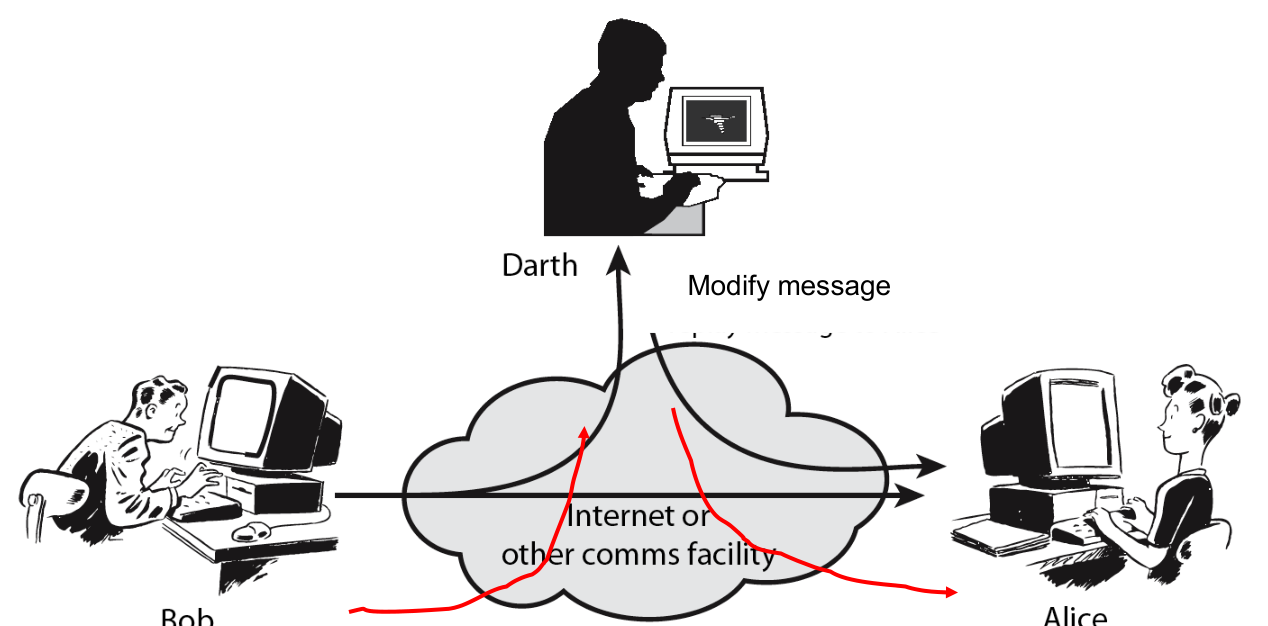
\includegraphics[width=138.60mm,height=172.26mm]{images/llm/page_048_img_01.png}%
\end{textblock*}

\newpage

% --- unit llm 49 ---
% === Halaman 49 (llm) ===

\vspace{250.97mm}

\begin{center}
\Large Man-in-the-middle-attack
\end{center}

\vspace{10mm}

% deskripsi: Diagram ilustrasi serangan Man-in-the-middle yang menunjukkan seorang pengguna (User) dan situs web (Website) yang koneksi aslinya terputus dan dialihkan melalui penyerang (Attacker/Man in the middle) melalui koneksi baru.
% bbox normalisasi: [0.2010, 0.1110, 0.7960, 0.9560]
\begin{textblock*}{124.95mm}(42.21mm,32.97mm)
\noindent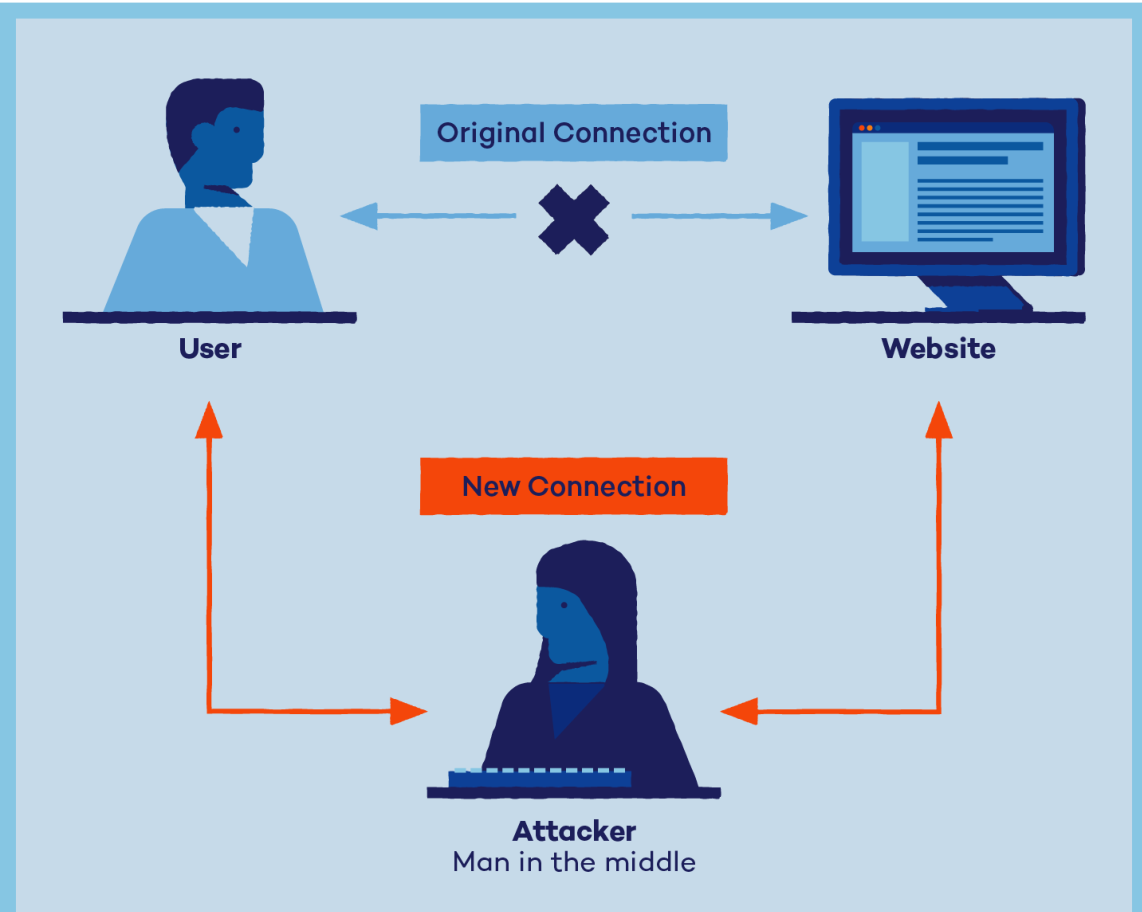
\includegraphics[width=124.95mm,height=250.97mm]{images/llm/page_049_img_01.png}%
\end{textblock*}

\newpage

% --- unit llm 50 ---
% === Halaman 50 (llm) ===

\vspace{196.02mm}

\begin{center}
\Huge Man-in-the-middle-attack
\end{center}

\vspace{20mm}

% deskripsi: Diagram alur serangan Man-in-the-Middle (MITM) pada proses pertukaran kunci Diffie-Hellman antara User A dan User B, menunjukkan bagaimana penyerang mengintersepsi dan memalsukan kunci publik.
% bbox normalisasi: [0.1500, 0.1700, 0.8100, 0.8300]
\begin{textblock*}{138.60mm}(31.50mm,50.49mm)
\noindent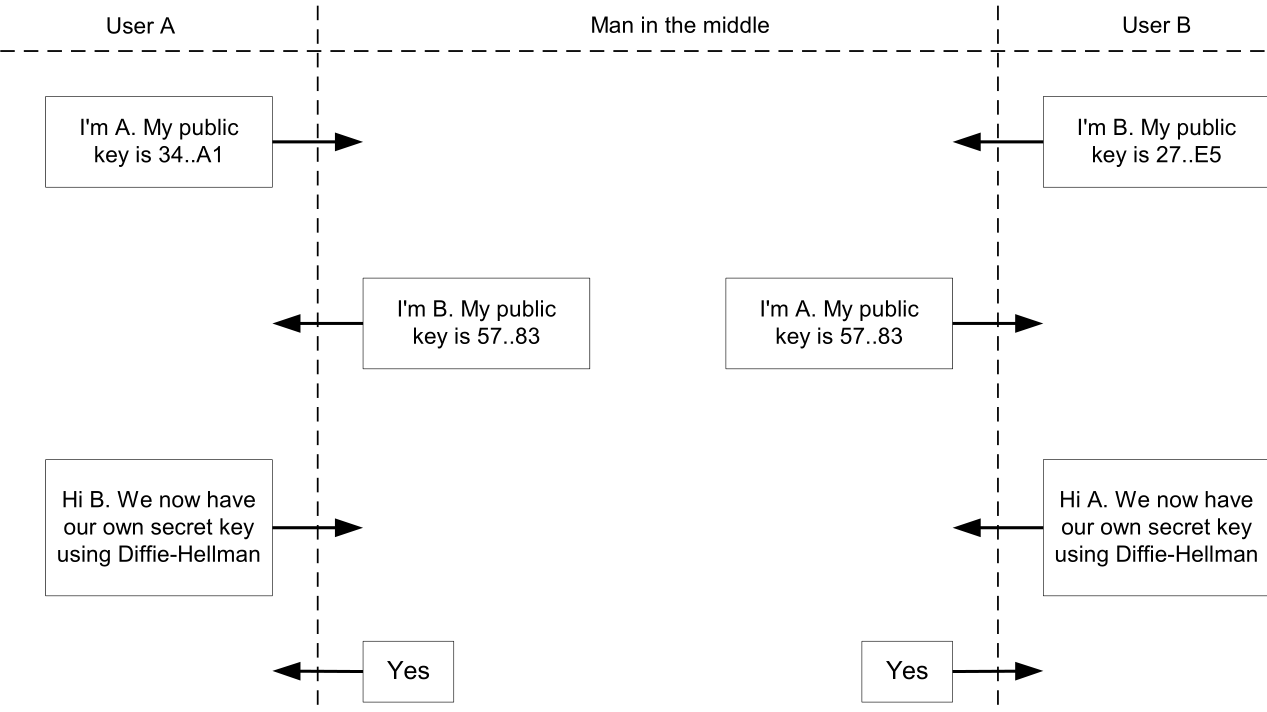
\includegraphics[width=138.60mm,height=196.02mm]{images/llm/page_050_img_01.png}%
\end{textblock*}

\newpage

% --- unit llm 51 ---
% === Halaman 51 (llm) ===

\begin{center}
\textbf{\large Man-in-the-middle-attack}\\
Serangan aktif yang berbahaya
\end{center}

\vspace{10mm}

% deskripsi: Diagram yang mengilustrasikan cara kerja serangan Man-in-the-Middle (MITM), menunjukkan interupsi koneksi asli antara User/Victim dan Web Application oleh penyerang (Man in the Middle).
% bbox normalisasi: [0.1700, 0.2600, 0.8900, 0.8500]
\begin{textblock*}{151.20mm}(35.70mm,77.22mm)
\noindent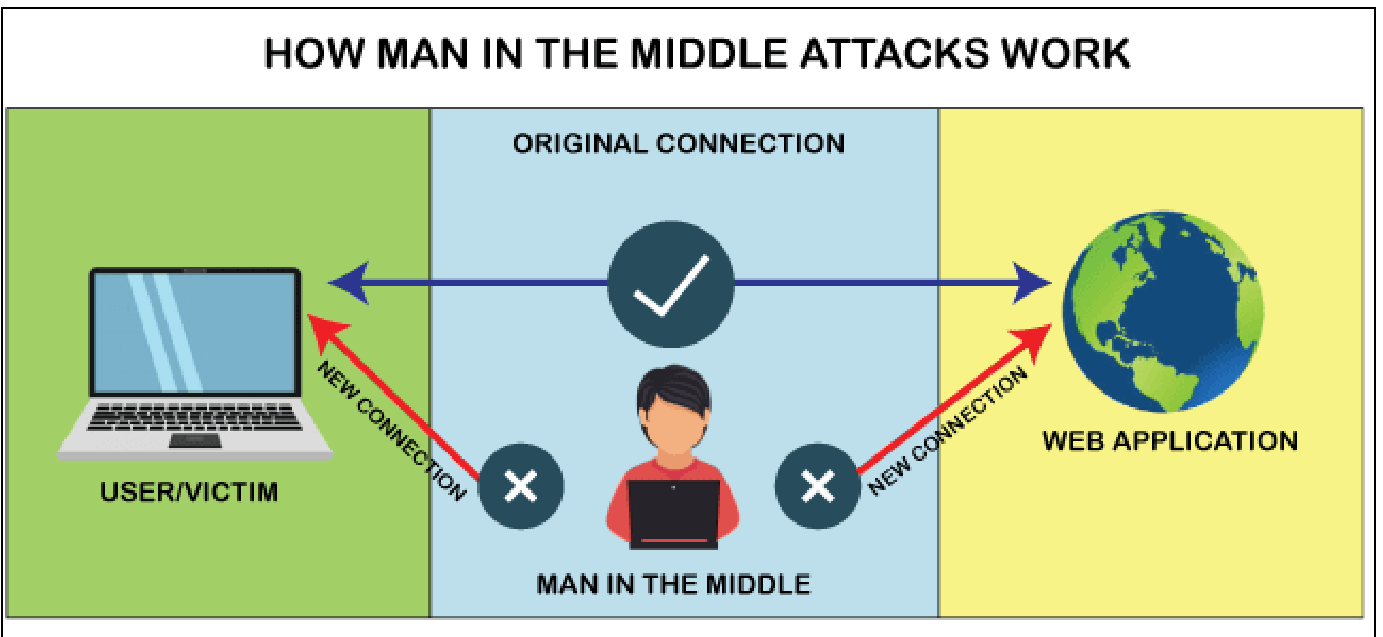
\includegraphics[width=151.20mm,height=175.23mm]{images/llm/page_051_img_01.png}%
\end{textblock*}

\newpage

% --- unit llm 52 ---
% === Halaman 52 (llm) ===

\section*{Serangan lainnya: Side-Channel Attack}

\begin{itemize}
    \item Serangan ini tidak terutama menyerang algoritma matematisnya, tetapi memanfaatkan informasi yang bocor ketika algoritma dijalankan pada perangkat fisik.
    \item Ada beberapa macam side-channel attack:
    \begin{enumerate}
        \item \textbf{Timing Attack} \\ Memanfaatkan perbedaan waktu eksekusi untuk memperoleh informasi tentang kunci.
        \item \textbf{Power Analysis Attack} \\ Menganalisis konsumsi daya perangkat ketika melakukan operasi kriptografi. Contohnya:
        \begin{itemize}
            \item Simple Power Analysis (SPA)
            \item Differential Power Analysis (DPA)
        \end{itemize}
        \item \textbf{Electromagnetic (EM) Attack} \\ Menganalisis radiasi elektromagnetik yang dihasilkan perangkat ketika melakukan operasi kriptografi.
        \item \textbf{Fault Injection Attack} \\ Penyerang sengaja menyebabkan kesalahan pada perangkat atau proses komputasi, kemudian menganalisis \textit{output} yang salah tersebut. Salah satu contohnya adalah Differential Fault Analysis (DFA).
    \end{enumerate}
\end{itemize}

\end{document}
